

\documentclass[DM,authoryear,toc]{lsstdoc}
% lsstdoc documentation: https://lsst-texmf.lsst.io/lsstdoc.html

% Package imports go here.
\usepackage{hyperref}
\usepackage{graphicx}
% Local commands go here.

% To add a short-form title:
% \title[Short title]{Title}
\title{Coaddition Artifact Rejection and \texttt{CompareWarp}}

% Optional subtitle
% \setDocSubtitle{A subtitle}

\input{authors}

\setDocRef{DMTN-080}
\setDocUpstreamLocation{\url{https://github.com/lsst-dm/dmtn-080}}
\setDocDOI{10.71929/rubin/2583441}

\date{2018-08-31}

% Optional: name of the document's curator
% \setDocCurator{The Curator of this Document}

\setDocAbstract{%
LSST images will be contaminated with transient artifacts, such as optical ghosts, satellite trails, and cosmic rays, and with transient astronomical sources, such as asteroid ephemerides.
We developed and tested an algorithm to find and reject these artifacts during coaddition, in order to produce clean coadds to be used for deep detection and preliminary object characterization.
This algorithm, \texttt{CompareWarpAssembleCoadd}, uses the time-series of PSF-matched warped images to identify   transient artifacts.
It detects artifact candidates on the image differences between each PSF-matched warp and a static sky model.
These artifact candidates include both true transient artifacts and difference-image false positives such as difficult-subtract-sources and variable sources such as stars and quasars.
We use the feature that true transients appear at a given position in the difference images in only a small fraction (configurable) of visits, whereas variable sources and difficult-to-subtract sources appear in most difference images.
In this report, we present a description of the method and an evaluation using Hyper SuprimeCam PDR1 data.
}

% Change history defined here.
% Order: oldest first.
% Fields: VERSION, DATE, DESCRIPTION, OWNER NAME.
% See LPM-51 for version number policy.
\setDocChangeRecord{%
  \addtohist{1}{2018-08-31}{Initial Version. \url{https://doi.org/10.5281/zenodo.2605418}.}{Yusra AlSayyad}
}

\begin{document}

% Create the title page.
% Table of contents is added automatically with the "toc" class option.
\maketitle


% ADD CONTENT HERE
\section{Introduction}
The annual Data Release Processing (DRP) will combine the multi-epoch images from LSST to extract the maximum information to support static-sky science.
One of the steps in DRP is coaddition:  resampling the images to a common projection,  normalizing them, and stacking them to produce a deeper image.
These resultant coadds will be used for various purposes throughout the pipelines: for deep detection, for initial object characterization, and as templates of the static sky from which each single-epoch exposure will be subtracted in the alert production process.
Therefore, coadds need to both cleanly represent the static sky and  maintain well-defined point spread functions (PSFs) for initial object characterization.

What is a clean representation of the static sky, given that the sky is not static?
First, every source detected on the coadd should still be at the detected position when followed-up with a spectrograph.
Second, variable stars and quasars should appear to have their ``average'' flux.
This average flux will depend on the cadence of the observations, of course.
To create a clean representation of the static sky, then, we must remove both the obvious non-astrophysical artifacts like ghosts, glints, satellites, cosmic rays, and chip defects (Figure \ref{fig:NineExamples}),  as well as the astrophysical temporal transients such as supernovae and asteroid ephemerides.\footnote{The distinction between transient and persistent sources is ambiguous for some cadences and objects.
Take, for example, an m-dwarf that, for most of the survey, is below the single-epoch detection limit, but that flares to 5$\sigma$ its quiescent luminosity---enough to be detected in one image.
In this case, the flare is not part of the static sky, and leaving it in the coadd would mean that the average flux of the source would be biased high.
If the flare is not included in the coadd, it will be more likely to be detected by image differencing during Alert Production.
Therefore, not only are transient flares of static objects treated as ephemeral because they are indistinguishable from transients and ephemerides, but it is also desirable to identify them during Alert Production for rapid follow-up.}


\begin{figure}
\begin{centering}
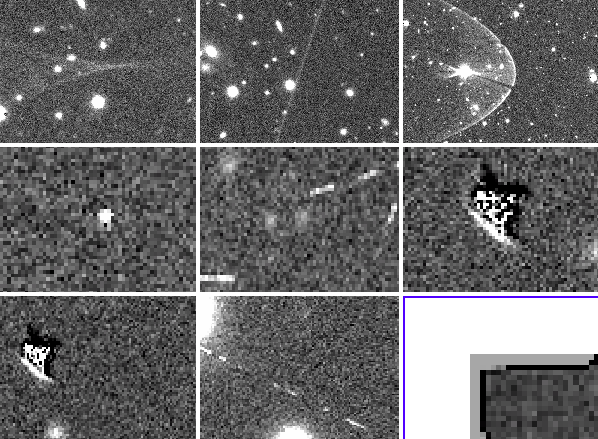
\includegraphics[width=0.8\textwidth]{figures/9examples.png}
\par\end{centering}
\caption{\label{fig:NineExamples} Nine examples of artifacts in HSC \texttt{directWarps} to be masked and removed. From the top left to bottom right they are (1) a ghost (2) a satellite (3) a ghost (4, 5)  cosmic rays (6, 7) chip defect group (8) cosmic ray, and (9) the unmasked edge of a sensor.}
\end{figure}

\begin{figure}
\begin{centering}
\includegraphics[width=0.6\textwidth]{figures/example4.png}
\par\end{centering}
\caption{\label{fig:safeclip} A ``SafeClipped'' (left), mean (middle) and sigma-clipped coadd (right), from ticket HSC-1166. The safeClip algorithm performed well on large, non-overlapping artifacts like these. It solved two problems with the sigma-clipped coadds: the visible wings of artifacts and artifacts falling within the $5\sigma$ (default) threshold with few numbers or epochs. Because SafeClipped used in an intermediate-stage a sigma-clipped coadd with a 1.5$\sigma$ threshold, it could clip artifacts even with low number of visits.}
\end{figure}

\begin{figure}
\begin{centering}
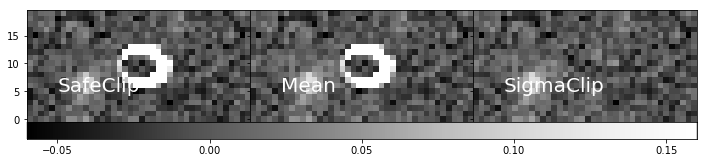
\includegraphics[width=0.6\textwidth]{figures/safeClip1.png}
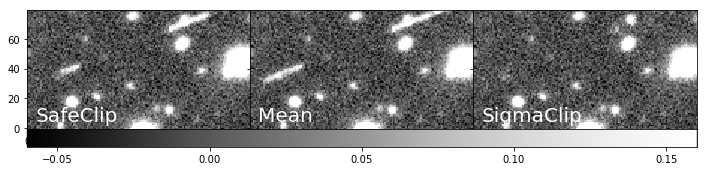
\includegraphics[width=0.6\textwidth]{figures/safeClip2.png}
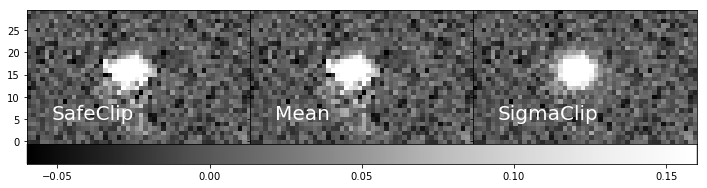
\includegraphics[width=0.6\textwidth]{figures/safeClip3.png}
\par\end{centering}
\caption{Three examples of SafeClip failure modes: a cosmic ray (top), asteroid (middle), chip defect group (bottom). Small overlapping artifacts like these persist in the SafeClip Coadd (left).  A clean coadd would look like the sigma-clipped coadd (right) rather than a raw mean (middle). \label{fig:safeClipExamples}}
\end{figure}

In prototype versions of the LSST software stack, we removed artifacts by using a per-pixel sigma-clipped mean as the stacking statistic.
However, coadds using this statistic have problems, including magnitude-dependent PSFs and traces of the edges of artifacts; an example of this can be seen in the right-hand panel of figure \ref{fig:safeClipExamples}.
In the summer 2013 development cycle, we improved artifact rejection with an algorithm we call ``SafeClip`` which produces ``SafeClipped Coadds.''
This algorithm was successful in removing large diffuse artifacts that appeared in only one epoch (figure \ref{fig:safeclip}).


However, to clip an artifact, the SafeClipped algorithm required that the artifact does not overlap with a real source and that it only appears in one epoch; therefore, the algorithm failed to clip asteroids that overlap in multiple epochs or chip defects that overlapped with static sources.
Figure  \ref{fig:safeClipExamples} shows a chip defect, a cosmic ray, and an asteroid that were not clipped by the SafeClipped algorithm.

The SafeClipped Coaddition algorithm differenced each visit with the sigma-clipped coadd and masked the pixels that had large deviations.
But the visits used for the differencing, called \texttt{directWarps}, have varying PSFs, and extreme seeing variations can appear as artifacts.
\texttt{directWarps} are simply the single-epoch visits resampled to the coadd pixel grid, and are described in more detail in Section \ref{sec:inputs}.

We build on this work, now using PSF-homogenized \texttt{psfMatchedWarps} for differencing.
\texttt{psfMatchedWarps} have been convolved with a matching kernel that transforms the PSF to a constant model PSF.
They can be subtracted from each other and a PSF-Matched Coadd more cleanly.
Proper PSF-matched warps became available in Spring 2017, and in Fall 2017, we implemented a new coaddition algorithm, called \texttt{CompareWarpAssembleCoadd}, which finds artifacts by inspecting the differences in the PSF-matched warps.

This algorithm uses the time axis to remove transients, and therefore it strictly targets transient artifacts without removing persistent artifacts.
Some examples of each:

Transient artifacts (to be rejected from coadds):
\begin{itemize}
\item Optical ghosts of bright stars\footnote{Ghosts can be large enough to present as additional ``background.'' In the future, we will evaluate when it is appropriate to subtract the ghost rather than mask it.} (these are consistent for a given pointing and rotator angle, and are persistent in snaps\footnote{one of the two exposures LSST expects to take at a given pointing} but not in warps).
\item Satellite trails, meteors
\item Glints (the reflection of starlight off of chip edges)
\item Cosmic rays
\item CCD defects (e.g., defect groups, bad columns)
\item Astrophysical transients (supernovae, asteroids), which are not part of the "static sky"
\end{itemize}

Persistent artifacts (to be treated elsewhere in software):
\begin{itemize}
\item Saturation bleed trails (persistent in surveys without rotational dithers)
\item Diffraction spikes (persistent in surveys without rotational dithers)
\item Cores of saturated stars
\item Astrophysical variable sources (variable stars, quasars)
\end{itemize}

As of January 2018, the \texttt{CompareWarpAssembleCoadd} algorithm is in production on the Hyper Suprime-Cam (HSC) S18A data release processing.
We discuss how this algorithm works in Section \ref{sec:method} of this technote, and we present the results of an evaluation of this algorithm on HSC data in Section \ref{sec:evaluation}.

\section{Algorithm to Mask Artifacts}
\label{sec:method}

\begin{figure}
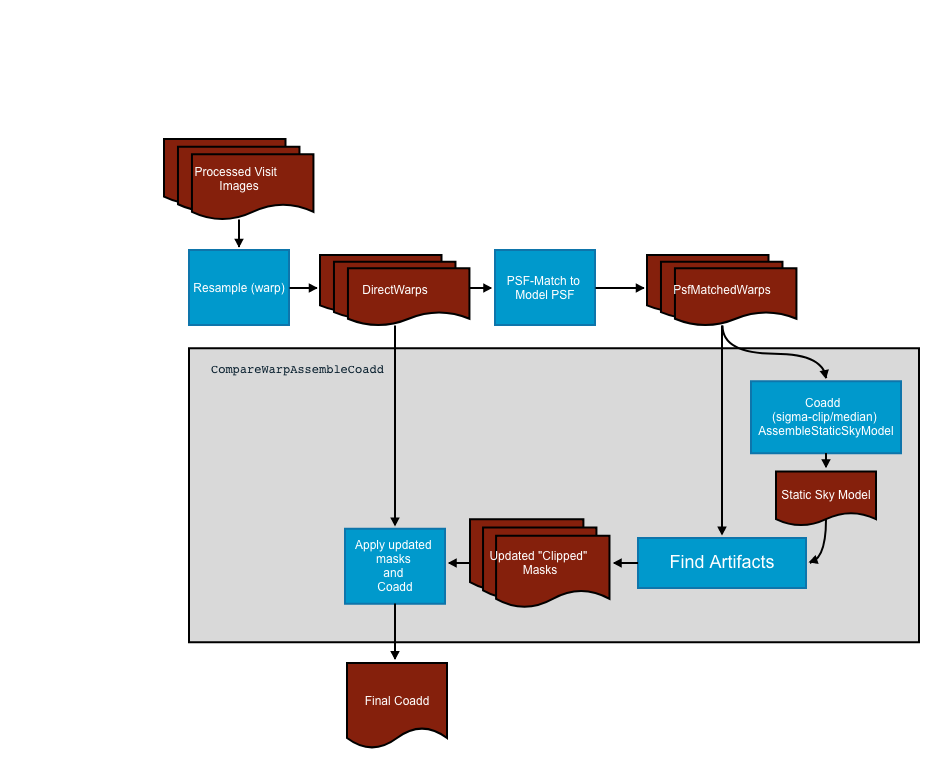
\includegraphics[width=1.0\textwidth]{figures/CompareWarpFlow.png}
\caption{Flowchart of the \texttt{CompareWarp} coaddition algorithm.\label{fig:flowchart} Red boxes represent data products with butler datatypes parentheses.  Blue boxes represent processing steps. The grey backgrounds represent the Tasks responsible.  Currently the updated artifact masks are used immediately when stacking the final coadds, but  we may store these as intermediate data products in the future.}
\end{figure}



The \texttt{CompareWarpAssembleCoadd} algorithm compares warps taken at different epochs to find and mask temporal artifacts.
In this section, we describe in more detail the artifact rejection method used by \texttt{CompareWarpAssembleCoadd}, summarized in figure \ref{fig:flowchart}.

\subsection{Inputs}
\label{sec:inputs}

During Data Release Processing we plan to make a three flavors of coadds \citep{DMTN-015}.
\begin{itemize}
\item Direct Coadd: Stack of images with no change to their PSFs.
\item  PSF-Homogenized Coadd: Stack of images after they have been reconvolved to a common, constant PSF
\item  Likelihood Coadd: optimal coadd stacked from images that have been convolved with the transpose of their PSFs
\end{itemize}

 \texttt{CompareWarpAssembleCoadd} can assemble coadds of all flavors.
 By default, it creates direct coadds, and in this example, we describe the inputs required to make the default direct coadds.
To make a direct coadd, \texttt{CompareWarpAssembleCoadd} requires two data products, \texttt{directWarps}, to be stacked, and \texttt{psfMatchedWarps}, to be compared for artifact detection.
\texttt{CompareWarpAssembleCoadd}  assumes that both data products have already been generated in the prior step, \texttt{makeCoaddTempExp}.
This prior step resamples (warps) the single-epoch images (also known as \texttt{calexps} or ``Processed Visit Images'') to a standard coadd geometry.
The smallest unit in this geometry is called a patch, an image that is small---usually a couple thousand by a couple thousand pixels---and easy to work with in memory.
Coadds and warps are both stored as one fits image per patch.

Direct warps have been resampled to a common pixel grid.
PSF-matched warps have been resampled to a common pixel grid and then convolved by a matching kernel that homogenizes their PSF to a constant model PSF, with the default model PSF being a Double Gaussian \citep{LDM-151}.
The best FWHM of the target model PSF depends on the data, specifically the seeing distribution of the input epochs.
We recommend the 90th--99th percentile of seeing.
Matching to a FWHM close to the maximum in the data minimizes the number of visits that are matched to a smaller PSF  and require a deconvolution which produces a noisier match.

\subsection{Make Static Sky Model}

Given these inputs, \texttt{CompareWarpAssembleCoadd} starts to find artifacts by generating a naive, artifact-free model of the static sky.
Because this model of the sky will be used only to find artifacts, an algorithm that destroys the PSF, such as a per-pixel median or sigma-clipped mean, is sufficient.
By default, \texttt{CompareWarpAssembleCoadd} generates a PSF-matched, sigma-clipped mean coadd as its naive model of the static sky, which it will compare to the individual PSF-matched warps.

In sections \ref{sec:detect}, \ref{sec:criteria}, \ref{sec:masks} we describe the subsequent steps of finding and labeling artifact candidates with this static sky model and PSF-matched warps.
A schematic of this procedure is shown in figure \ref{fig:demo}.
Figures \ref{fig:demo}, \ref{fig:artifacts}, and \ref{fig:countMap} demonstrate the steps for patch=``6,4'', a 4200 x 4200 pixel area of the COSMOS field (tract 9813) taken with HSC, which have warps from 33 $i$-band visits.
In this example, we matched the PSFs of each visit to a Double Gaussian with a FWHM of 7.7 pixels (1.3 arcseconds).
This corresponds to the 98th percentile of seeing for all 5 bands for WIDE-survey observations taken before April 2018.

\subsection{Detect Artifact Candidates}
\label{sec:detect}

\begin{figure}
\begin{centering}
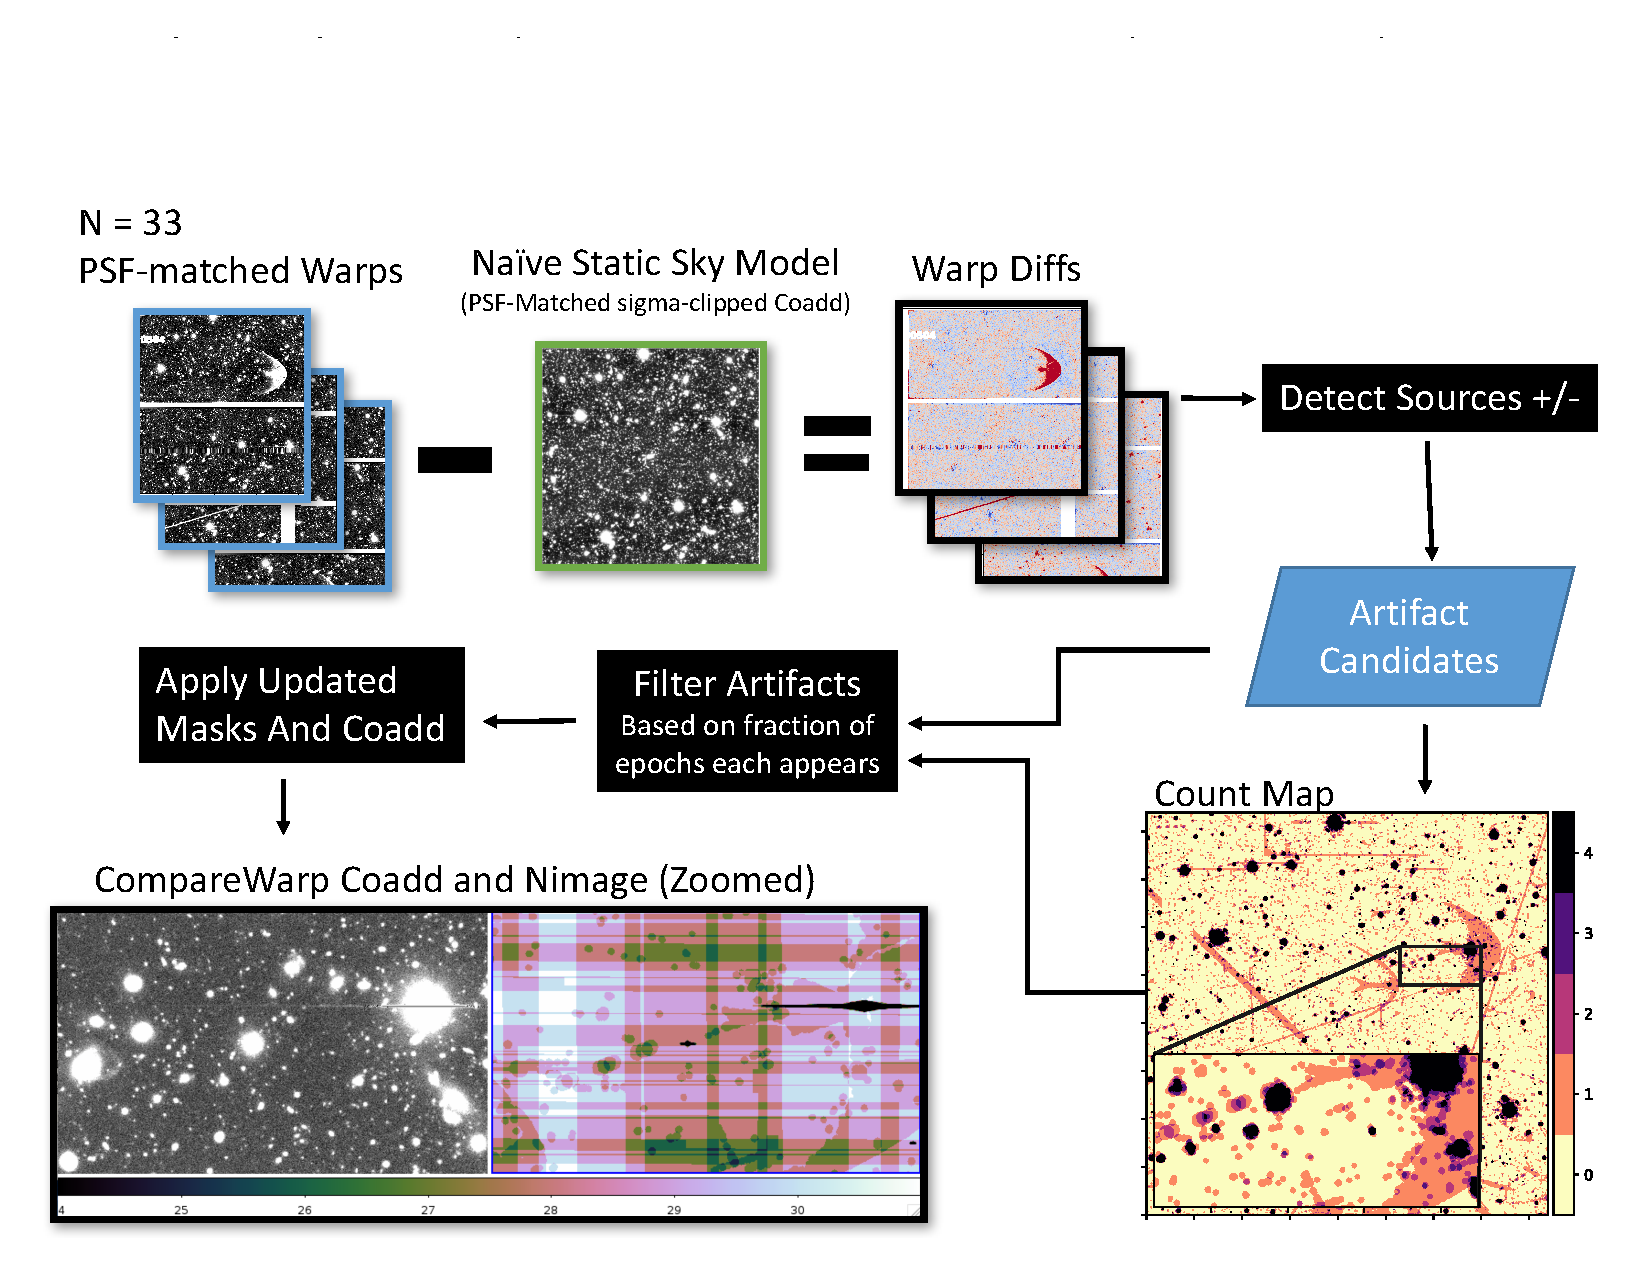
\includegraphics[width=0.75\textwidth]{figures/CompareWarpDemo.pdf}
\par\end{centering}
\caption{\label{fig:demo} Sketch of the steps performed by \texttt{CompareWarpAssembleCoadd} for tract=9813, patch=``6,4'', filter=``HSC-I''.}
\end{figure}

To find artifacts, we subtract this static sky model from each PSF-Matched warp to produce a ``difference warp,'' or \texttt{WarpDiff}.
We then run our source detection algorithm, \texttt{SourceDetectionTask} on this difference warp to detect sources, both positive and negative.
This step generates a set of regions that are above or below the threshold; we call these regions \texttt{Footprints}, and they identify areas where the epoch/visit deviates more than 5$\sigma$ (this value is configurable) from the naive static sky model.
These \texttt{Footprints} detected in the difference image can be thought of as ``residual'' or ``outlier'' flux.
They mark regions where the sky deviates from the Static Sky Model at a particular epoch.

Some of these detections are non-astrophysical temporal transients/artifacts that we want to mask (e.g. cosmic rays, chip defects, satellites and others in figure \ref{fig:artifacts}).
However, all image differencing processes produce false positives, and not all the detections are true transient artifacts.
The detections may also include variable stars and quasars or subtraction imperfections, such as dipoles, which are stars that are slightly offset in position for various reasons (differential chromatic diffraction, astrometric errors, or simple brightness).
\footnote{For any arbitrarily small astrometric offset, a sufficiently bright star will still produce a dipole in the difference image.}

\begin{figure}
\begin{centering}
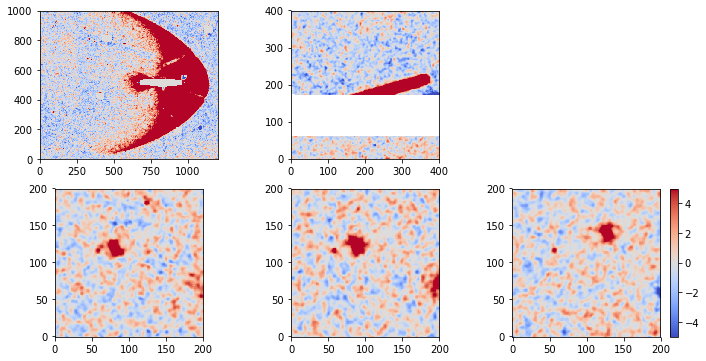
\includegraphics[width=0.6\textwidth]{figures/artifacts.png}
\par\end{centering}
\caption{\label{fig:artifacts} Image difference produced by subtracting the PSF-matched coadd from a PSF-matched Warp. The color scale is the image divided by the square root of the variance plane. Positive detections on the top row include a ghost from a bright star and a satellite trail. The bottom row shows one asteroid in three consecutive epochs/visits.}
\end{figure}

How do we separate these variable sources/subtraction imperfections from the true transients that we want to mask?
We can leverage one or both of the following attributes.
First, the vast majority of the subtraction imperfections are bright stars.
Since we know where the bright stars are from the first round of source measurement in single-visit processing, \texttt{processCcd}, we can ignore any artifact candidates near bright stars.
Second, we can distinguish between transient artifacts and subtraction imperfections because transient artifacts appear in one, two or three epochs, while subtraction imperfections appear in most epochs.
In other words, if an object is hard to subtract cleanly in one epoch, then it is hard to subtract in many.
This feature not only allows us to filter false positives but allows us to define ``transient'' as a source that appears in a configurable percentage of visits.
For this reason,  we use this second attribute in \texttt{CompareWarpAssembleCoadd}.

We produce a ``Count Map'' to record how many epochs each residual detection appears in.
As we loop through the  \texttt{WarpDiffs}, we accumulate a count map of the detected \texttt{Footprints}.
Figure \ref{fig:countMap} shows an example count map of the demo patch.
The large ghost of a bright star and asteroids appear only once or twice in the image, whereas bright stars are detected in the difference warp in almost every visit.

\begin{figure}
\begin{centering}
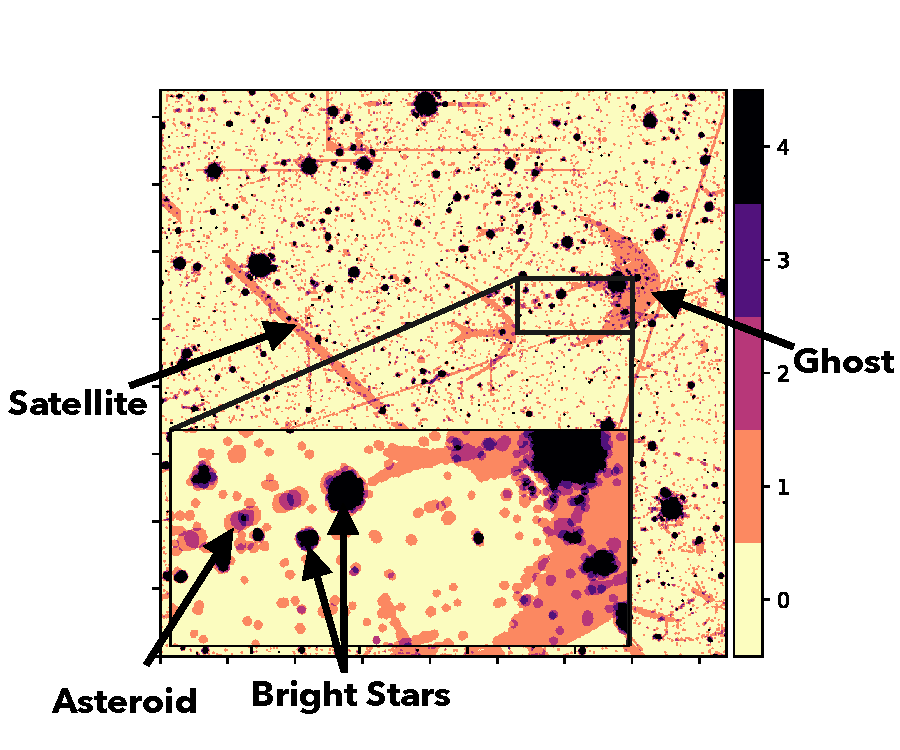
\includegraphics[width=0.85\textwidth]{figures/AnnotatedEpochCountImage.pdf}
\par\end{centering}
\caption{\label{fig:countMap} An \texttt{epochCountImage}:  Count of the number of epochs in which the  pixel is contained by a detection on a difference warp or of the number of epochs in which that pixel is part of an residual detection.  Real artifacts and transients appear only once or twice in the epoch count map, but subtraction imperfections appear in almost all epochs---25 or more of the 33 epochs.  The colormap was clipped at four to show the detail in the lower numbers. }
\end{figure}

\subsection{Masking Criteria for Artifact Candidates}
\label{sec:criteria}

At this stage, each detection in the \texttt{WarpDiff} is designated as an ``artifact candidate."
The artifact candidate pool is filtered by the count map, which provides the information to identify which artifact candidates are actual transients to be clipped and which are variable objects and subtraction imperfections.
If a significant fraction of a footprint's pixels is residual (above/below threshold) in a significant fraction of epochs, the footprint is not an artifact and should not be masked.
Configuration parameters in \texttt{CompareWarpAssembleCoadd} provide quantitative definitions of ``significant fraction of pixels''   (\texttt{config.spatialThreshold}) and ``significant fraction of epochs'' (\texttt{maxFractionEpochsLow}, \texttt{maxFractionEpochsHIgh}, \texttt{maxNumEpochs})

For each artifact candidate we compute the following quantities:
\begin{itemize}
\item \texttt{maxNumEpochs}, the temporal threshold of what constitutes a ``significant fraction of epochs.''
If more than half of the footprint appears in a number of epochs that is higher than this number, the footprint is labeled ``persistent.''
 If more than half the footprint appears in a number of epochs that is fewer than this number, the candidate is labeled ``temporal'' and is clipped.
 \texttt{maxNumEpochs} is a fraction of the average number of total epochs contributing to the footprint ($N$). For $N$ of 1 or 2, \texttt{maxNumEpochs} should be 0:  there is simply not enough information in one or two epochs to identify outliers.
For $N$ of 3 or 4, \texttt{maxNumEpochs} should be 1, and for $N=5$, up to 2 epochs can be clipped. For $N>5$,  \texttt{maxNumEpochs} is a very slow-growing fraction of $0.03N$, to accommodate coadds of up to hundreds of epochs.
\item  Fraction of pixels in the footprint where the epoch count is less than the \texttt{maxNumEpochs}.
\end{itemize}

The following pseudocode illustrates this temporal criterion.
For each artifact candidate footprint, we extract the \texttt{epochCountImage} (the object representing the Count Map described above) and the \texttt{nImage} (the number of total visits contributing to a pixel).
These cutouts are called \texttt{outlierN} and \texttt{totalN} respectively.
It computes the \texttt{maxNumEpochs} based on the configuration parameters and the mean number of visits contributing to that region (\texttt{totalN}).
If the fraction of pixels in that region having \texttt{outlierN} (outlier counts) less than  \texttt{maxNumEpochs} is less than the configurable spatial threshold (50\% by default), it is labeled a true transient artifact.
Otherwise, it is considered persistent and not masked for clipping.

\begin{verbatim}
def isArtifactCandidateTemporal(artifactSpanset)
    y, x = artifactSpanset.indices()
    outlierN = epochCountImage.array[y, x]
    totalN = nImage.array[y, x]
    maxNumEpochs = functionOf(config, mean(totalN))
    fractionBelowThreshold = count_nonzero(outlierN <= maxNumEpochs) / outlierN.size()
    return fractionBelowThreshold > config.spatialThreshold
\end{verbatim}


% Illustrate with  a couple of examples from visit 30504?

\subsection{Masks}
\label{sec:masks}
The footprints of artifact candidates that meet the temporal criteria above are designated as temporal artifacts and are passed to the final coaddition step to be clipped.
The final coaddition step uses the default coaddition algorithm with a mean stacking statistic: each pixel is computed to be the weighted mean of the input pixels, excluding any visits with ``bad'' mask bits set.
These bad mask bits include the new \texttt{CLIPPED} plane and modified \texttt{NO\_DATA} plane, both passed in from the artifact rejection procedure.

The coaddition procedure sets the \texttt{CLIPPED} bit and the  \texttt{NO\_DATA} bit in the the \texttt{directWarp} mask  based on the information it receives from the artifact rejection routine.
Any pixels in a \texttt{directWarp} that overlap an artifact have the \texttt{CLIPPED} mask plane set and are excluded while stacking.
The  \texttt{NO\_DATA} bit needs to be set too because PSF matched warps  have less usable data than direct warps.
PSF-matched warps have less area because they are convolved by an extra matching kernel.
Because we do not have any information for those pixels along the edge of the \texttt{calexps} in the PSF-matched warps, we must leave those pixels out by default.
For an example region, figure \ref{fig:nodata} shows the resulting coadds with \texttt{NO\_DATA} updated (left) versus \texttt{NO\_DATA} not updated (second from left).
The \texttt{PsfMatched} \texttt{warpDiff} (right)  has less area than the direct warp (second from right).
The integrated area will always be less for  \texttt{CompareWarpAssembleCoadd} because it uses PSF-matched warps for temporal information.

\begin{figure}
\begin{centering}
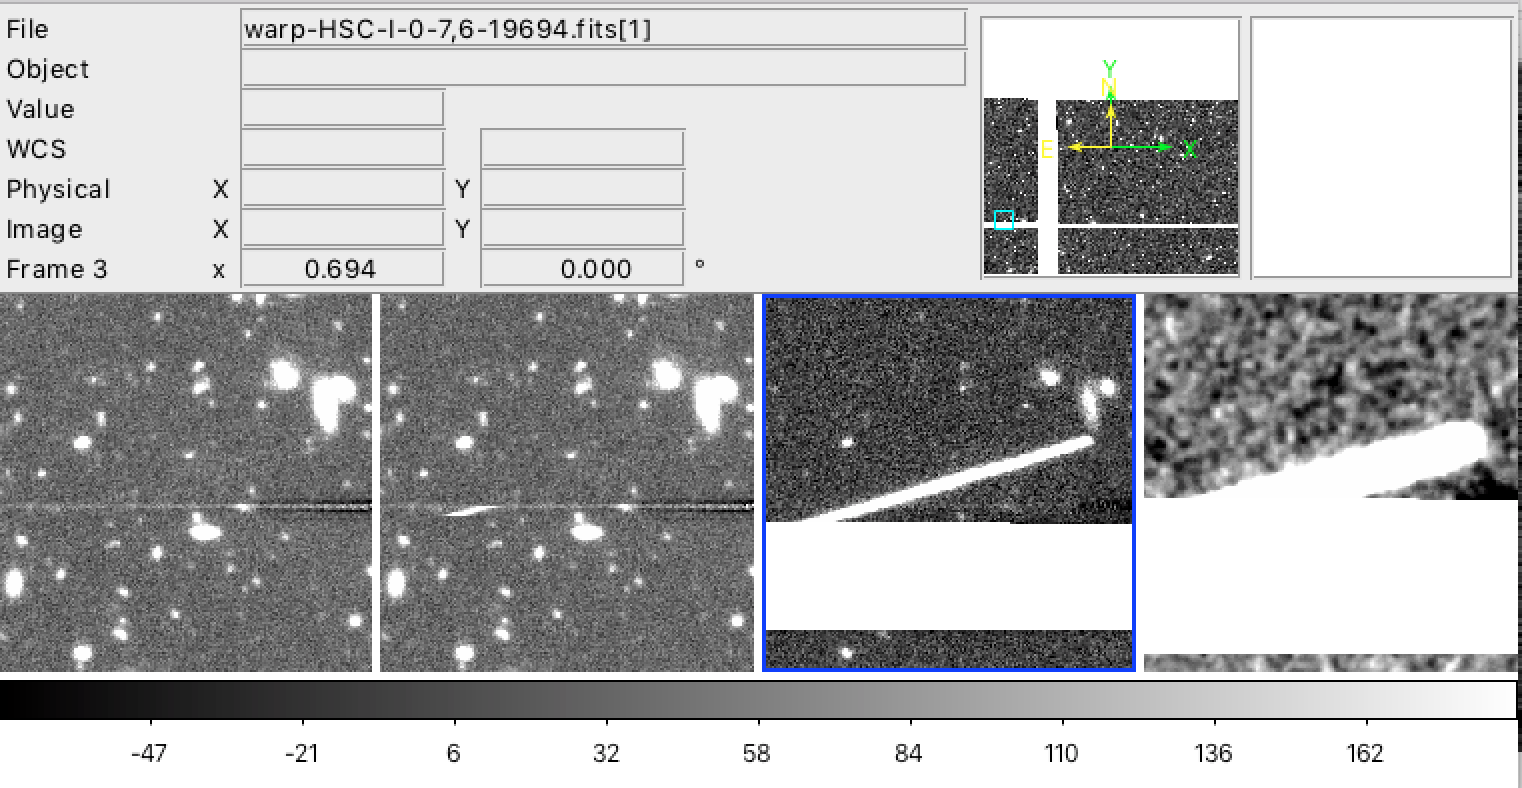
\includegraphics[width=0.6\textwidth]{figures/less_data.png}
\par\end{centering}
\caption{\label{fig:nodata}  Demonstration of why setting the \texttt{NO\_DATA} mask plane is necessary. The PSF-Matched warp diff (right panel) has less usable area for temporal comparison than the Direct Warp (third panel). Therefore we mark the absence of that information with the \texttt{NO\_DATA} to create the coadd in the first panel, or else we would end up with a coadd in the second panel.}
\end{figure}

\subsection{Comparison with other Algorithms}

\texttt{CompareWarpAssembleCoadd} is similar to the algorithm described by \citet{2016A&C....16...67D} and used by the Dark Energy Survey (DES), but it differs in a few major ways.
First, the static sky model in DES  is generated from a \emph{catalog} of sources measured on a median PSF-matched coadd.
In DES, the static sky model is realized in the visit projection (rather than in the coadd projection, as in \texttt{CompareWarpAssembleCoadd}) and is subtracted from the single-epoch images.
We did not use the approach of subtracting model sources from images because we do not assume that all light is either a  compact source or an artifact.
There are astrophysical sources such as ultra-diffuse galaxies and Galactic cirrus  that are not catalogued, but we nonetheless want to appear in the coadds at their full SNR.

Second, while we grow the detections on the \texttt{WarpDiff}s  based on  the width of the model PSF, \citet{2016A&C....16...67D} use an iterative approach.
They first run detection with a  5-sigma threshold,  then grow the detections to include the surrounding pixels that are above 2.5-sigma, and then make a final pass to grow the detections again, this time including surrounding pixels that are above 1.5-sigma,
in order to capture all the surrounding low-surface-brightness flux.
This may be worth trying after background matching as a way to clip very low-surface-brightness ghosts.

Third, we PSF-match to double Gaussian PSF models where they PSF-match to Moffat PSFs.
The target PSF model should not matter.

%Maybe compare to Gruen if I have time

\section{Evaluation}
\label{sec:evaluation}

\texttt{CompareWarpAssembleCoadd} was evaluated on a number of axes: run time, false positives, and false negatives.
We tested the algorithm on the HSC data release candidate dataset (RC2) which includes \textbf{3 tracts} from the public data release  described in \citet{2018PASJ...70S...5B}.

\begin{itemize}
\item Tract 9813: Ultra-deep (UD) COSMOS field  in filters: HSC-G, HSC-R, HSC-I, HSC-Z, HSC-Y and NB0921
\item Tract 9615: WIDE GAMA15H field  in filters: HSC-G, HSC-R, HSC-I, HSC-Z, HSC-Y
\item Tract 9697: WIDE VVDS field  in filters: HSC-G, HSC-R, HSC-I, HSC-Z, HSC-Y
\end{itemize}

In general, WIDE fields have 2--10 epochs, and the UD COSMOS field has tens of epochs, so this test set spans two orders of magnitude in numbers of epochs.
We also evaluated the algorithm on a few patches that included observations taken after the Public Data Release 1 (PDR1) in order to confirm that the algorithm could be extended to hundreds of epochs (ensuring that it could become public in a future HSC data release), but these evaluation results are not presented here.

Each tract includes 81 patches on a 9 by 9 grid.  Each patch is 4200x4200 pixels. We ran \texttt{coaddDriver.py} and \texttt{multibandDriver.py} with configurations summarized in table \ref{fig:reruns}.

\begin{table}
\footnotesize
\begin{center}
 \begin{tabular}{l l l l}
 rerun  & algorithm & \texttt{makeCoaddTempExp} configs  & configs \\
 \texttt{/private/yusra/RC2/*} &  & \texttt{doApplySkyCorr?}  & \texttt{assembleCoadd.*} \\
 \hline\hline
   \texttt{w\_2018\_18} & \texttt{CompareWarp} & True &  \\
   \hline
   \texttt{w\_2018\_18\_doNotApplySkyCorr} & \texttt{CompareWarp} & False &  \\
   \hline
 %  \texttt{w\_2018\_18\_doNotPreserveContained} & \texttt{CompareWarp} & False &  doPreserveContainedBySource=False  \\
  % \hline
   \texttt{w\_2018\_18\_wcNoBadAmp} & \texttt{CompareWarp} & False & doPrefilterArtifacts=False \\
   \hline
   \texttt{w\_2018\_18\_sigmaClip} & \texttt{AssembleCoadd}  & False &  \\
   \hline
   \texttt{w\_2018\_18\_safeClip} & \texttt{SafeClipCoadd}  & False &  \\
   \hline
\end{tabular}
\end{center}
\caption{\label{fig:reruns} Summary of rerun configurations. }
\end{table}

\texttt{w\_2018\_18} is the configuration used in the S18A internal HSC data release.
This data release was processed with a new Sky Correction algorithm which was designed to mitigate the over-subtraction of sky near bright stars and galaxies (https://community.lsst.org/t/sky-subtraction/2415).
However, most reruns were tested with the new Sky Correction \emph{off} via the config parameter \texttt{doApplySkyCorr=False}.
We found that the background offsets introduced by the sky correction interfered with the image differencing in both \texttt{CompareWarp} and  \texttt{SafeClip}.
We can better compare the performance of the algorithms without the additional effects of mismatched backgrounds.
See section \ref{sec:background_matching} for more information.

We included a rerun of \texttt{CompareWarp} with a non-default configuration, \texttt{w\_2018\_18\_wcNoBadAmp}, because it was the configuration used for coaddition in the S18 PDR1 reprocessing at NSCA, see \url{https://confluence.lsstcorp.org/display/DM/S18+HSC+PDR1+reprocessing} for more information.
Note that this internal PDR1 reprocessing did include the new sky correction \emph{on}, so it is not an exact representation of the PDR1 rerun.

Artifact rejection involves some trade-offs between cleanliness and depth.
We want to clip as many artifacts as possible  without degrading the signal-to-noise ratio and without clipping across too many sources, interfering with their PSFs.
In the limit of a large number of visits,   every source will fall on the edge of some chip gap or the edge of some artifact. For this reason, we are pursuing ideas to circumvent measuring sources on coadds, such as MultiFit or per-object coadds.
In the meantime, there are configuration parameters that control the aggressiveness of the artifact rejection algorithm.
%Link to discussion on config parameters.

We verify depth (false positives/over-clipping) through the QA metrics on the PSF photometry.
Too many clipped sources will present as an increase in the scatter of the stellar locus.

We verify cleanliness (false negatives/under-clipping) by measuring usable survey area and comparing detections on coadds from each rerun with those detected on the sigma-clipped coadds; sigma-clipped coadds stand in for a truth catalog.
% False negatives can also appear as reduced SNR if a large ghost is unclipped and degrades the photometry or prevents the deblending of the sources behind it.


\subsection{Photometry (False Positives/Over-clipping)}

We ran a DRP with 5 configurations, and used \texttt{colorAnalysis} in the  \texttt{pipe\_analysis} package to compute and plot the stellar locus in each. For the full set of plots, see \url{lsst-web.ncsa.illinois.edu/~yusra/artifact_rejection/dmtn-080}.
For example, figure \ref{fig:wFit} shows the $g-r$ vs. $r-i$ PSF-magnitude colors for compact sources as produced by  \texttt{pipe\_analysis} for  rerun= \texttt{w\_2018\_18\_doNotApplySkyCorr} (top) and rerun= \texttt{w\_2018\_18\_sigmaClip} (bottom).
The scatter in the stellar locus is caused by a combination of variance in the natural colors of stars (from e.g. metallicity differences) and measurement errors.
Therefore, a robust measurement of the width of the stellar locus is a proxy for photometric repeatability.
We compare the metric labeled here as wPerp$_\mathrm{wired}$ std. between reruns.

\begin{figure}
\begin{centering}
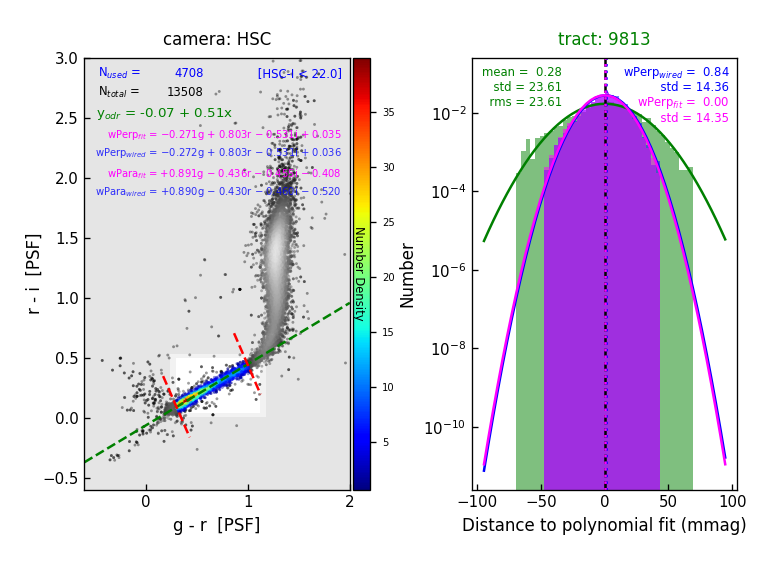
\includegraphics[width=0.75\textwidth]{figures/plot-t9813-griPSF-wFit-fit.png}
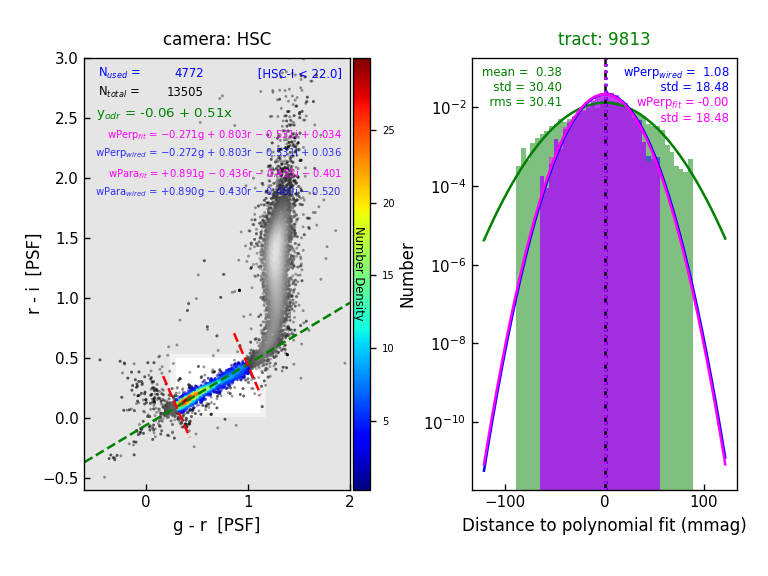
\includegraphics[width=0.75\textwidth]{figures/plot-t9813-griPSF-wFit-fit-sigmaClipped.png}
\par\end{centering}
\caption{\label{fig:wFit}  Two example stellar locus plot output by \texttt{colorAnalysis.py} in the \texttt{pipe\_analysis} package for tract=9813 and rerun= \texttt{w\_2018\_18\_doNotApplySkyCorr} (top) and  \texttt{w\_2018\_18\_sigmaClip} (bottom) The metric compared between reruns is labeled here as wPerp$_\mathrm{wired}$std=14.35 mmag for CompareWarp and 18.48 for sigmaClip.  For CompareWarp In the top panel, this value is approximately equal to the intrinsic width of the stellar locus and therefore indicates good stellar photometry because minimal additional scatter was introduced by photometric errors. For the SigmaClipped coadds (bottom), the width is unacceptably high.}
\end{figure}

Figure \ref{fig:w_std_fit} compares the width of the $g-r$ vs $r-i$ stellar locus,  the robust standard deviation of the stars perpendicular distance from the locus ($w2$ color per \cite{2004AN....325..583I}).
Lower numbers are better.
The leftmost configuration \texttt{CompareWarp\_skyCorr\_on} is the default configuration used in the S18A HSC data release.
All other configurations shown do not use the new sky correction.
The second configuration from the left, uses the default CompareWarp configuration but with the new sky correction turned off.

The stellar photometry is better \emph{without} the new sky correction step, especially in the UD COSMOS tract 9813.
CompareWarp performs better for all tracts than does SafeClip in terms of stellar photometry.
We confirm, as shown in QA on previous data challenges, that sigma-clipping produces poor stellar photometry and is exactly the reason we do not use per-pixel sigma clipping for coaddition.

\begin{figure}
\begin{centering}
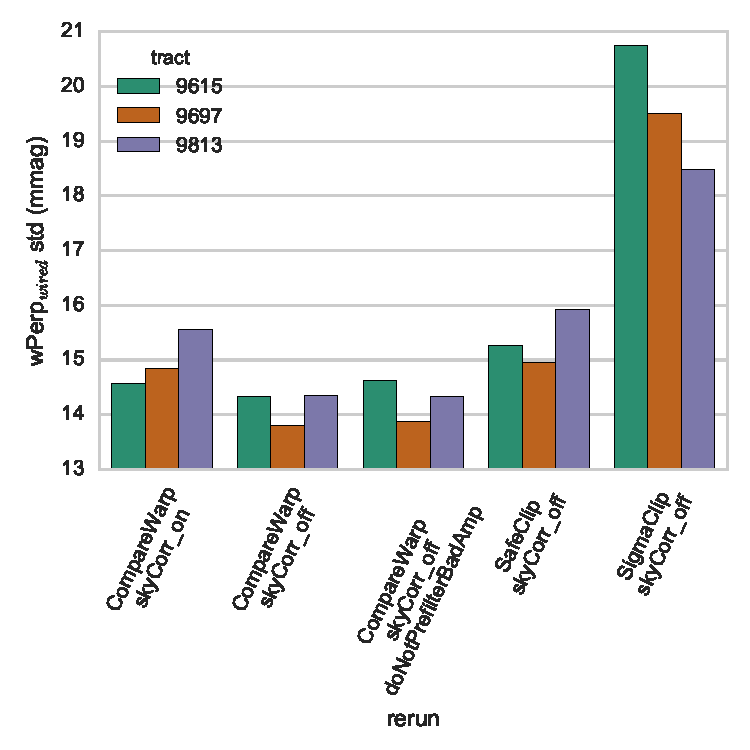
\includegraphics[width=0.9\textwidth]{figures/w_std_fit.pdf}
\par\end{centering}
\caption{\label{fig:w_std_fit} Width of the $g-r$ vs $r-i$ stellar locus for the 3 tested tracts and 5 configurations (reruns). Lower numbers are better. The statistic shown is the robust standard deviation of the a star's perpendicular distance from the stellar locus (its $w2$ color defined in \cite{2004AN....325..583I}). \texttt{CompareWarp}, the new algorithm presented in this technote, performs better than both SafeClip and the per-pixel sigma-clipped coadds on all three tracts. All reruns except the left-most, have had the HSC SkyCorrection turned off. }
\end{figure}

\subsection{Unclipped artifacts (False Negatives/Under-clipping)}

False negatives, artifacts that were unclipped, can manifest in two ways.
First, compact artifacts appear as additional detections, relative to "truth."
For example, unclipped asteroids and comic rays will appear as extra catalog sources.
Second, extended artifacts can appear as spatial gaps in the source catalogs because they are large footprints that cannot be properly deblended.
For example, unclipped ghosts and glints will appear as gaps in the source catalogs.
We present metrics for both types of false negatives.

\textbf{Unclipped Extended Artifacts}:
We compute survey area at the catalog level to quantify the area contaminated by ghosts.
Large numbers are better/cleaner.
Regions contaminated by ghosts are empty of sources and we use a void-finding algorithm,  sometimes referred to as an alpha-hull algorithm.
We first compute the Delauney triangulation of the  $> 5\sigma$ sources.
Every edge between two adjacent sources contributes to exactly two triangles.
Triangles with a circumference larger than a tunable threshold are pruned from the full set of triangles.
The remaining edges that appear in the triangulation only once form the boundary of the  survey area.
The vertices of the holes (edges that only appear once in the set) comprise mask polygons.
We compute both the area of these polygons and the remaining survey area using the Python package \texttt{Shapely}.
We use vertices in R.A. and Dec. coordinates with distances in R.A./Dec. space which means that the absolute survey ares does not take into account the curvature of the sky.
However,  because we only care about the \emph{relative} usable area comparing different reruns of the same part of the sky, these effects are canceled out.

% Demo for 9813, patch 8,2

\begin{figure}
\begin{centering}
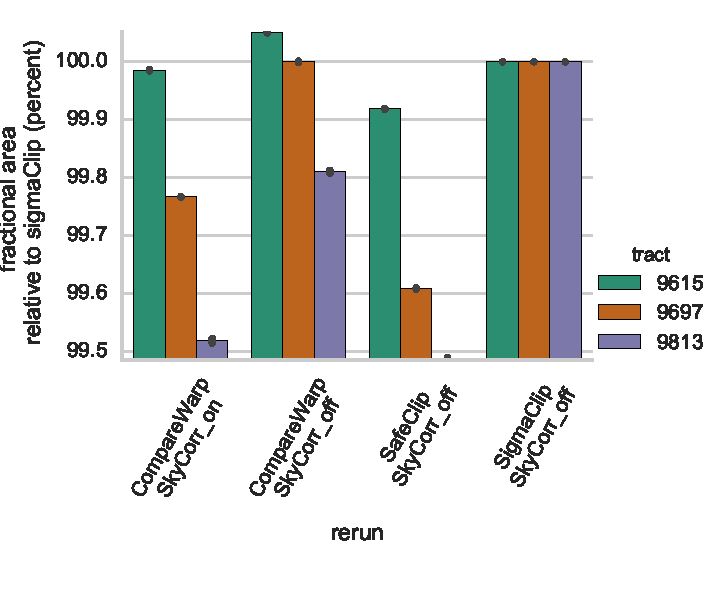
\includegraphics[width=0.7\textwidth]{figures/survey_area.pdf}
\par\end{centering}
\caption{\label{fig:area} Coadd survey area computed per filter and tract relative to survey area computed for the sigma-clipped coadd with the SkyCorr turned off.  Larger numbers (percentages) are better.  The fraction for \texttt{SigmaClip} is 100\% by definition. The CompareWarp algorithm performs the best for all tracts, and even \emph{better} than sigma-clipped for tract 9615.  Again, artifact rejection in general performs better with the sky correction turned off. }
\end{figure}

Figure \ref{fig:area} shows the computed survey area computed per filter and tract.
The quantity displayed is $100A_{r,f,t}/A_{r=\mathrm{sigmaClip}, f,t}$ where $f$ represents a specific filter and $t$ a specific tract, $r$ a rerun, averaged over all filters for a tract/rerun combination.  This fractional area for rerun=sigmaClip, is 100\% by definition. Larger numbers are better because they represent more usable area.

Comparing the two apples-to-apples reruns CompareWarp and SafeClip both with the sky correction turned off, we see CompareWarp yields more usable area (fewer contaminated regions).
The difference is more significant for the ultra deep tract 9813 and tract 9697.
CompareWarp actually performed better than sigma-clipped for the wide tract 9615.
This is possible because the default threshold for the sigma-clipped algorithm is $\sigma=5$, and the threshold for the template of the static sky used by \texttt{CompareWarp} is a lower $\sigma=2.5$.

\textbf{Unclipped Compact Artifacts}: Second, compact artifacts appear as surplus detections, relative to a "truth catalog."
Whereas we do not have a truth catalog, we define the default sigma-clipped coadd as ``truth,'' and define an unclipped artifact as follows.
For each rerun, tract, and bandpass, we concatenate the \texttt{deepCoadd\_meas} tables of all 81 patches.
\texttt{deepCoadd\_meas} tables are the single-band coadd measurements of the merged detections---the union of detections in all 5 bands.
We then select the sources that have a psfFlux SNR > 5, the \texttt{detect\_isPrimary} flag set, and the ``qaBad'' flag not set.
We then look for sources that do not have a match within 1 arcsecond of the same catalog in the ``sigmaClip'' rerun (which has only been filtered for \texttt{detect\_isPrimary}).

Not all the matchless sources are unclipped artifacts however. Visual inspection shows that most are close to the detection limit and the coadded images are mostly identical, with minor differences in a background offset or a few pixels (<10\%)  that were sigma clipped.
We therefore also require a matchless source to have a significantly different coadd image in the 25x25 pixel bounding box around the centroid, where significantly different is defined as
\begin{equation}
1.1 < \chi^2_{\nu} = \frac{1}{N-1}\sum^{N}_{i=1} \frac{{(x_i - y_i)}^2}{\sigma_x^2 + \sigma_y^2}
\end{equation}
where $x_i$ is a pixel in the coadd being evaluated and $y_i$ is the corresponding pixel on the sigma-clipped coadd.
Some $\chi^2$ values are significant only because of a background offset. Backgrounds of sigma-clipped coadds are systematically lower than those of ``SafeClipped,'' ``CompareWarp'' or mean coadds.
Therefore, we also require that a $\chi^2$ of the mean scaled differences:
\begin{equation}
0.35 < \chi^2_{\nu-matched} = \frac{1}{N-1}\sum^{N}_{i=1} \frac{{(x_i - y_i  + \bar{y} - \bar{x})}^2}{\sigma_x^2 + \sigma_y^2}.
\end{equation}

Figure \ref{fig:uniquePosDet} compares this metric for false-negatives (unclipped artifacts) in each of the reruns, passbands, and tracts.
In all tracts and bands, ``CompareWarp'' performed better than ``SafeClip'' on this metric, especially so for the tracts and bands with more visits.
Again, the artifact rejection performed better on the rerun with the new sky correction disabled.

\begin{figure}
\begin{centering}
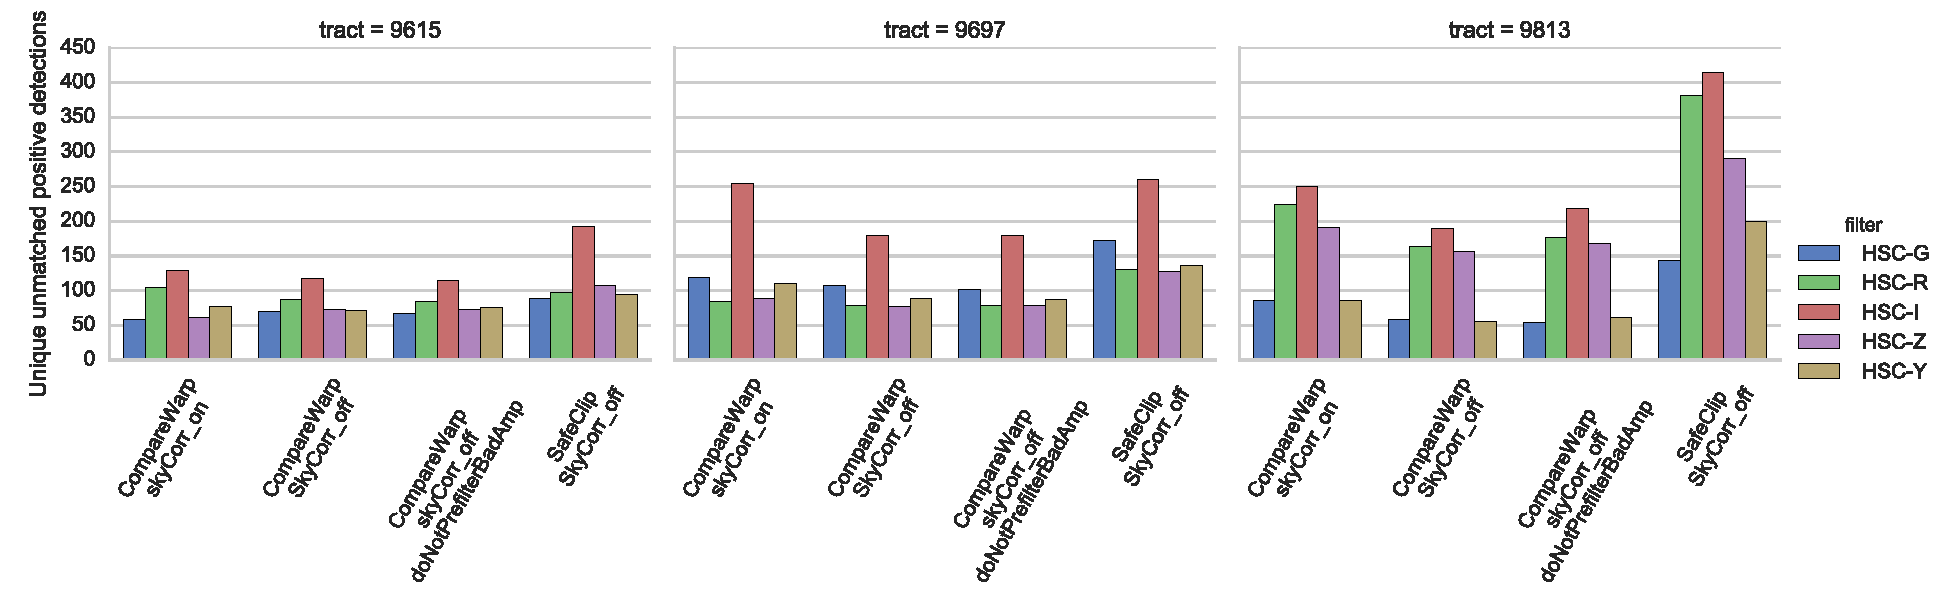
\includegraphics[width=1.0\textwidth]{figures/missed_uniquePosDet.pdf}
\par\end{centering}
\caption{\label{fig:uniquePosDet} Unique unmatched positive detections. Lower values are better. CompareWarp performs better in by this metric especially for the coadds with more visits.}
\end{figure}

\subsection{Examples of Behavior}
Figure \ref{fig:old_examples} displays two examples taken from the evaluation dataset to demonstrate that \texttt{CompareWarp} successfully clips different types of transient artifacts.

\begin{figure}
\begin{centering}
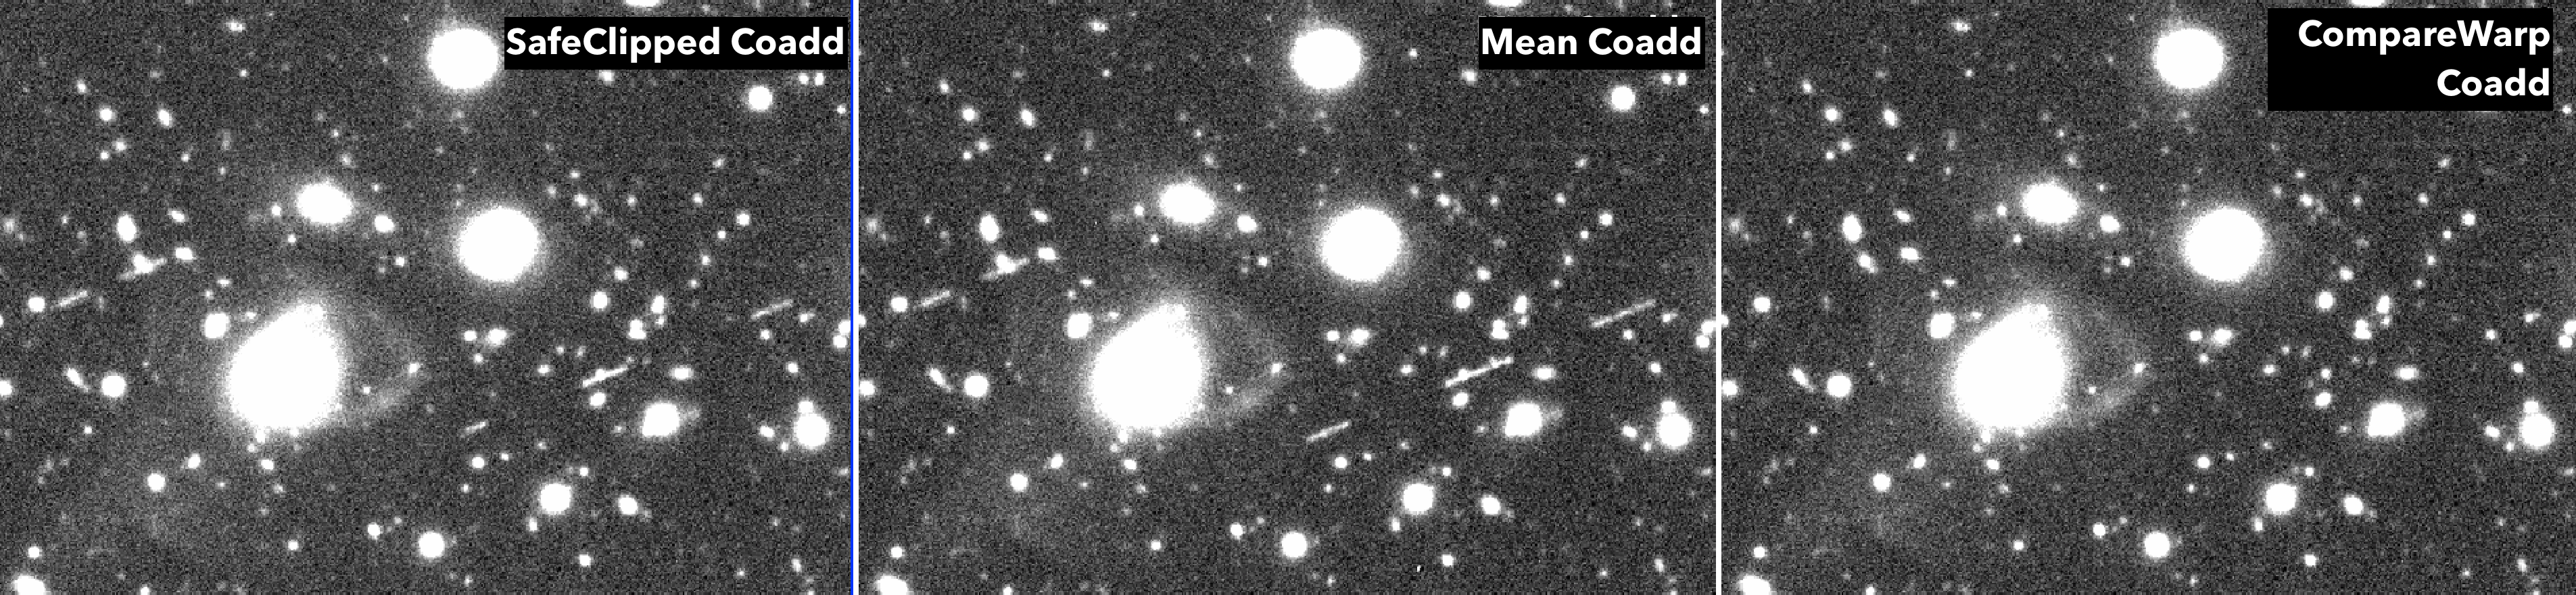
\includegraphics[width=0.9\textwidth]{figures/prototypeRobustAsteroids.png}
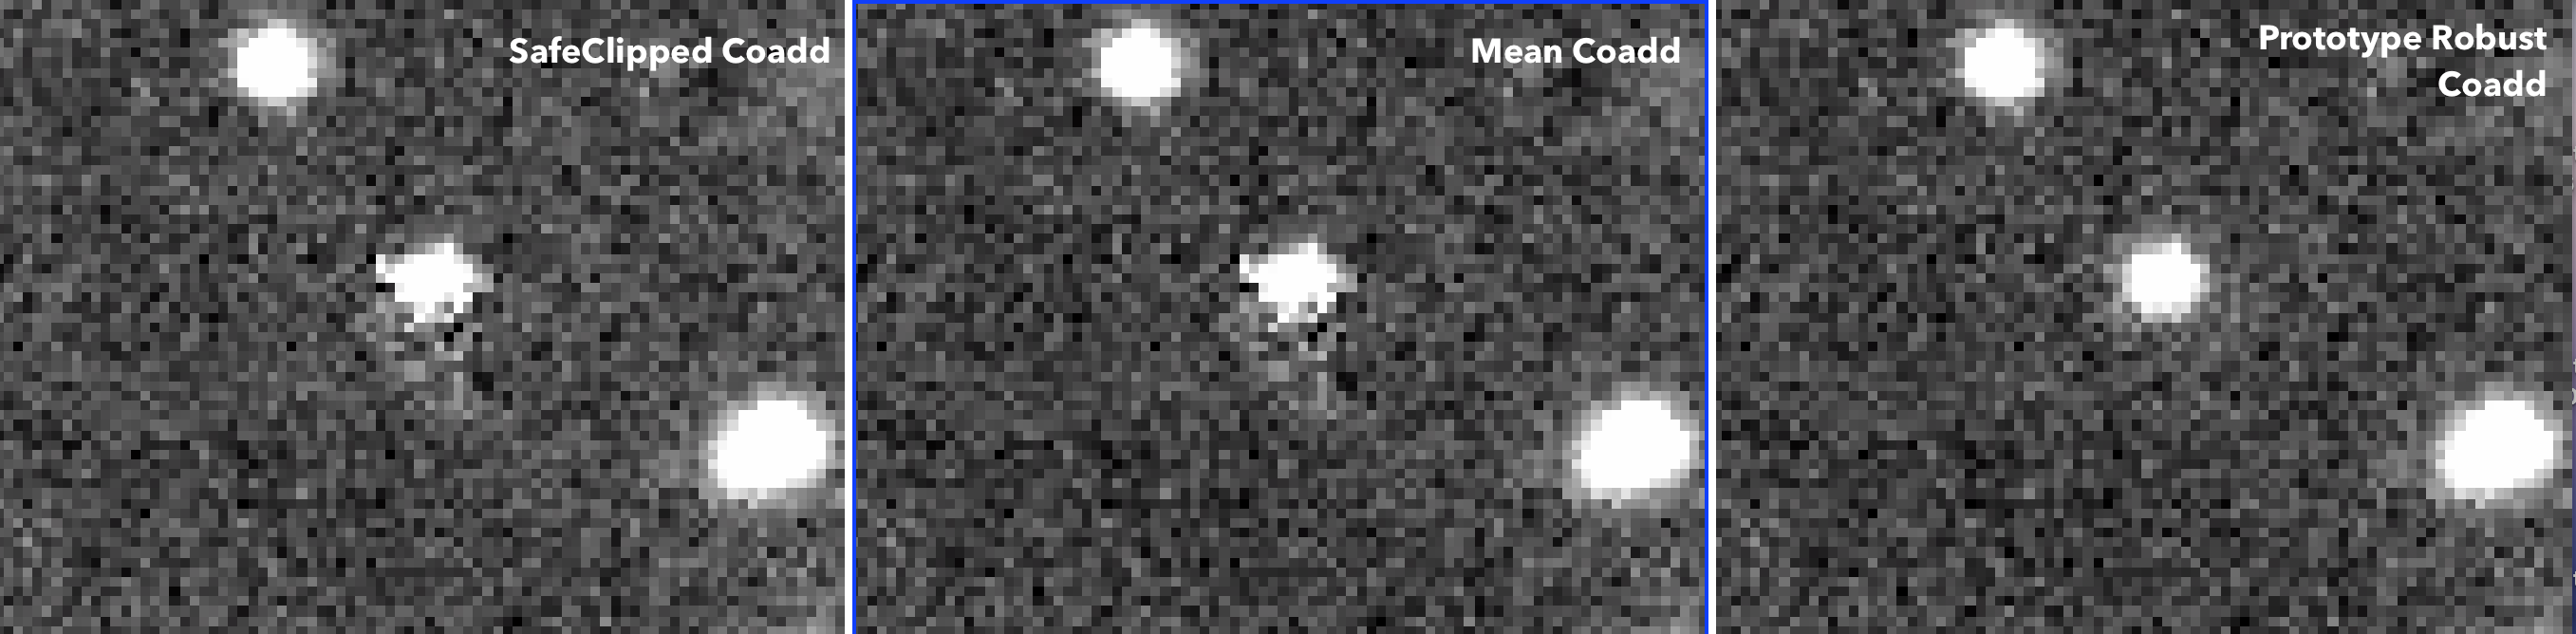
\includegraphics[width=0.9\textwidth]{figures/PrototypeRobustDetect1.png}
\par\end{centering}
\caption{\label{fig:old_examples} Two examples of artifacts that SafeClip found challenging: an overlapping sequence of asteroids (top) and a defect group that lands on a star (bottom).  A "Mean Coadd" (center; for comparison) uses no artifact rejection.  \texttt{SafeClipped} (left) removes the outer most asteroids of each of the overlapping series, but  \texttt{CompareWarp} (Right)  removes all asteroids in the overlapping series.}
\end{figure}


\subsection{Runtime}
A full data release  production \texttt{CompareWarpAssembleCoadd} takes longer to run because it relies on PSF-matched warps, and PSF matching requires an extra convolution on each warp.
These convolutions are currently the bottleneck in runtime.
The runtime of the assembling procedure itself is comparable to that of the SafeClip algorithm.

\subsection{Failure Modes}

\textbf{Under-dithered Surveys}: If a survey is not dithered sufficiently, it can create coincident ghosts and coincident CCD defects.
For example, a moustache-like ghost appears in half the visits (figure \ref{fig:underdithered}).
This makes it show up in the static sky model, and because it is in the static sky model, it cannot be detected as a temporal artifact.

\begin{figure}
\begin{centering}
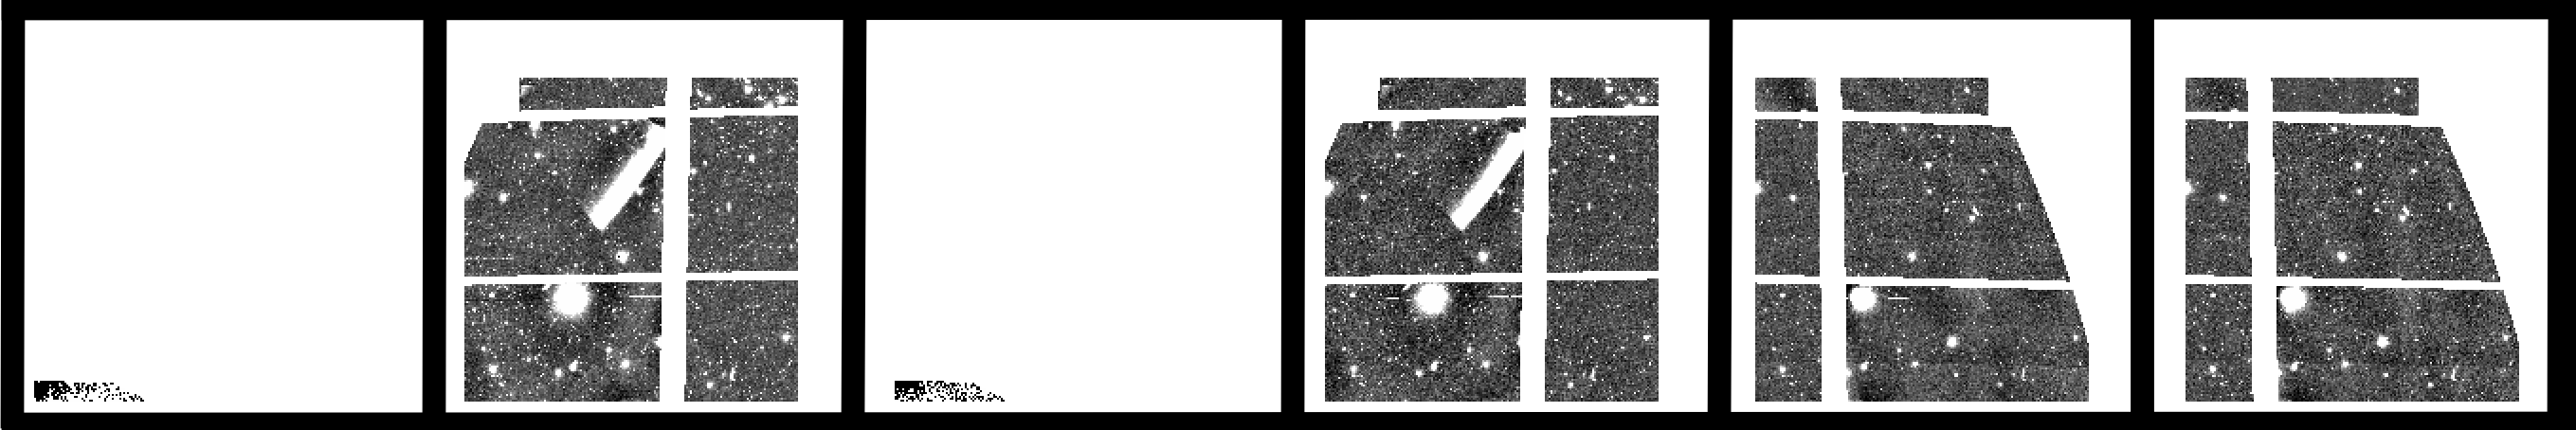
\includegraphics[width=0.9\textwidth]{figures/underdithered.png}
\par\end{centering}
\caption{\label{fig:underdithered} Six PSF-matched warps that repeat observations at the same pointings. The bright artifacts, which the HSC collaboration calls mustaches, in the second and fourth warps are impossible to clip because they appear in half the epochs with coverage.}
\end{figure}

This is especially apparent in the UD COSMOS field 9813.
Figure \ref{fig:9813Maps} shows the pixels in the resulting coadd that have any epoch clipped.
In the HSC-Z band image on the right,  there is a gap in the clipping in the bottom left-hand corner of the tract in patch 1,2.
Because there are so many overlapping artifacts in this region,  the algorithm reads them all as persistent, and as a result, none of them get clipped.

\begin{figure}
\begin{centering}
\begingroup
\sbox0{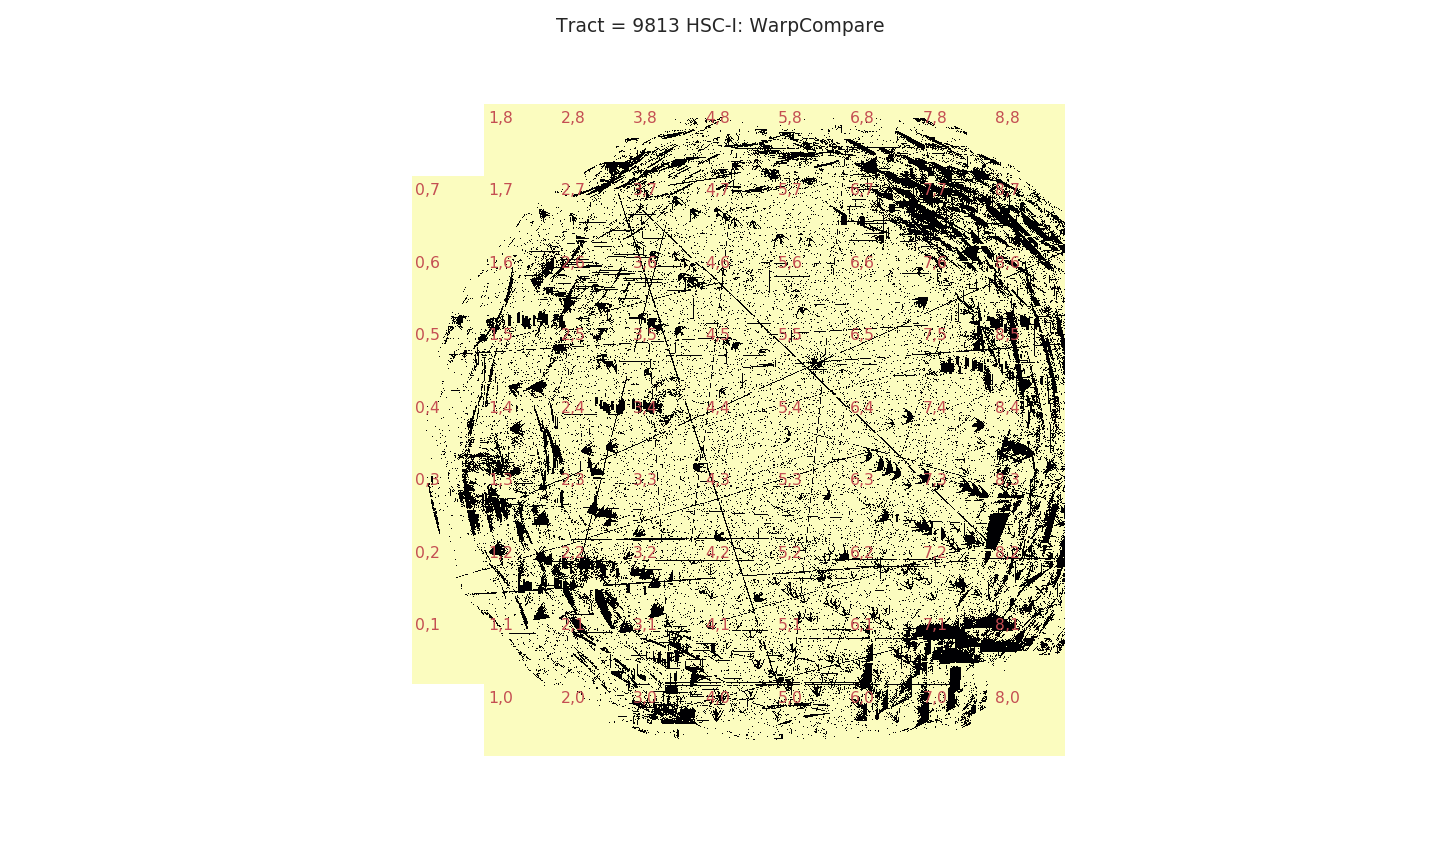
\includegraphics{figures/mask_DM-13637_9813HSC-I.png}}%
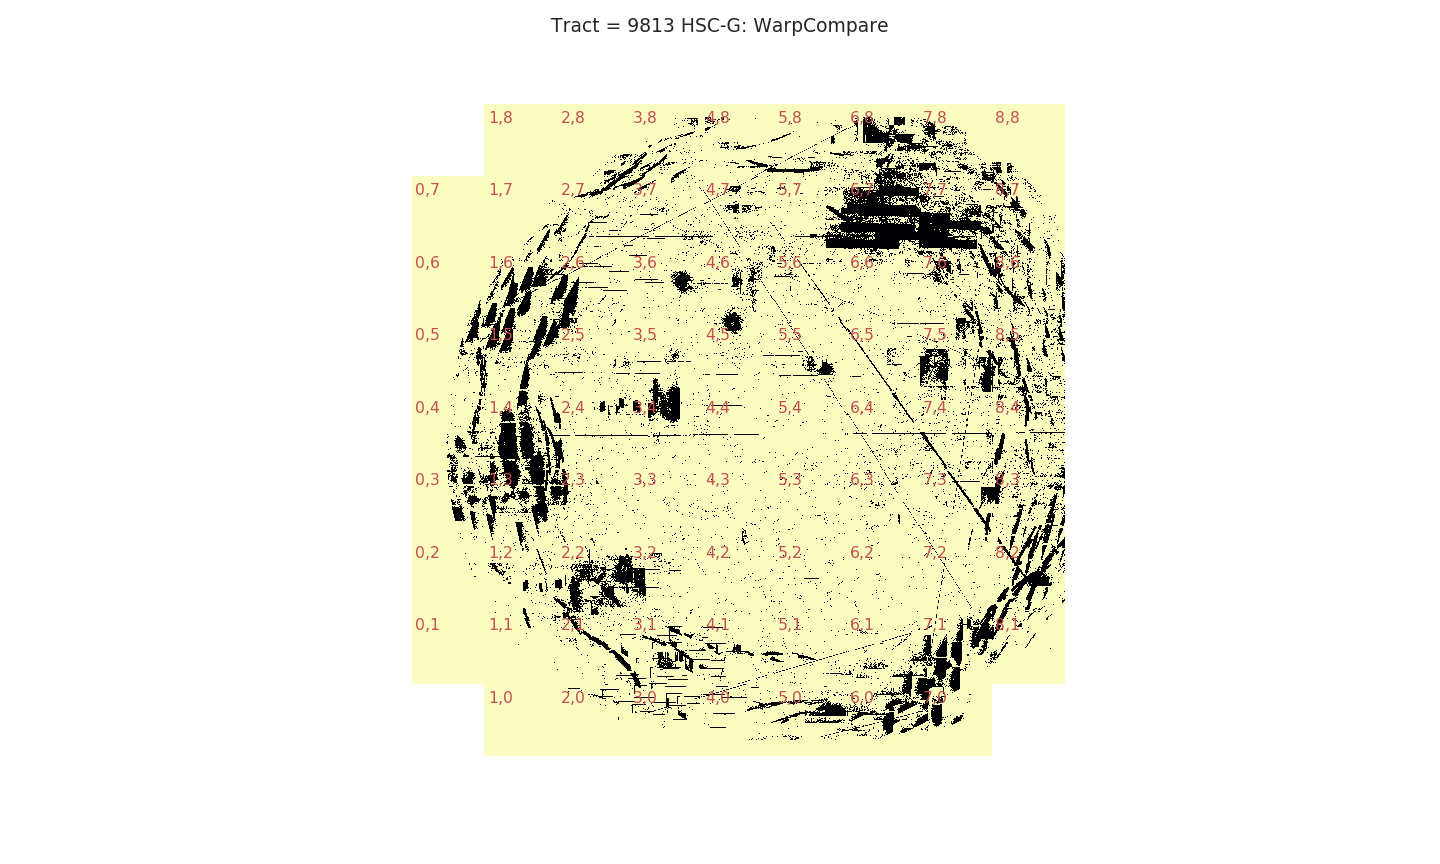
\includegraphics[clip,trim={.25\wd0} {.05\wd0} {.25\wd0} 0, width=0.30\textwidth]{figures/mask_DM-13637_9813HSC-G.png}
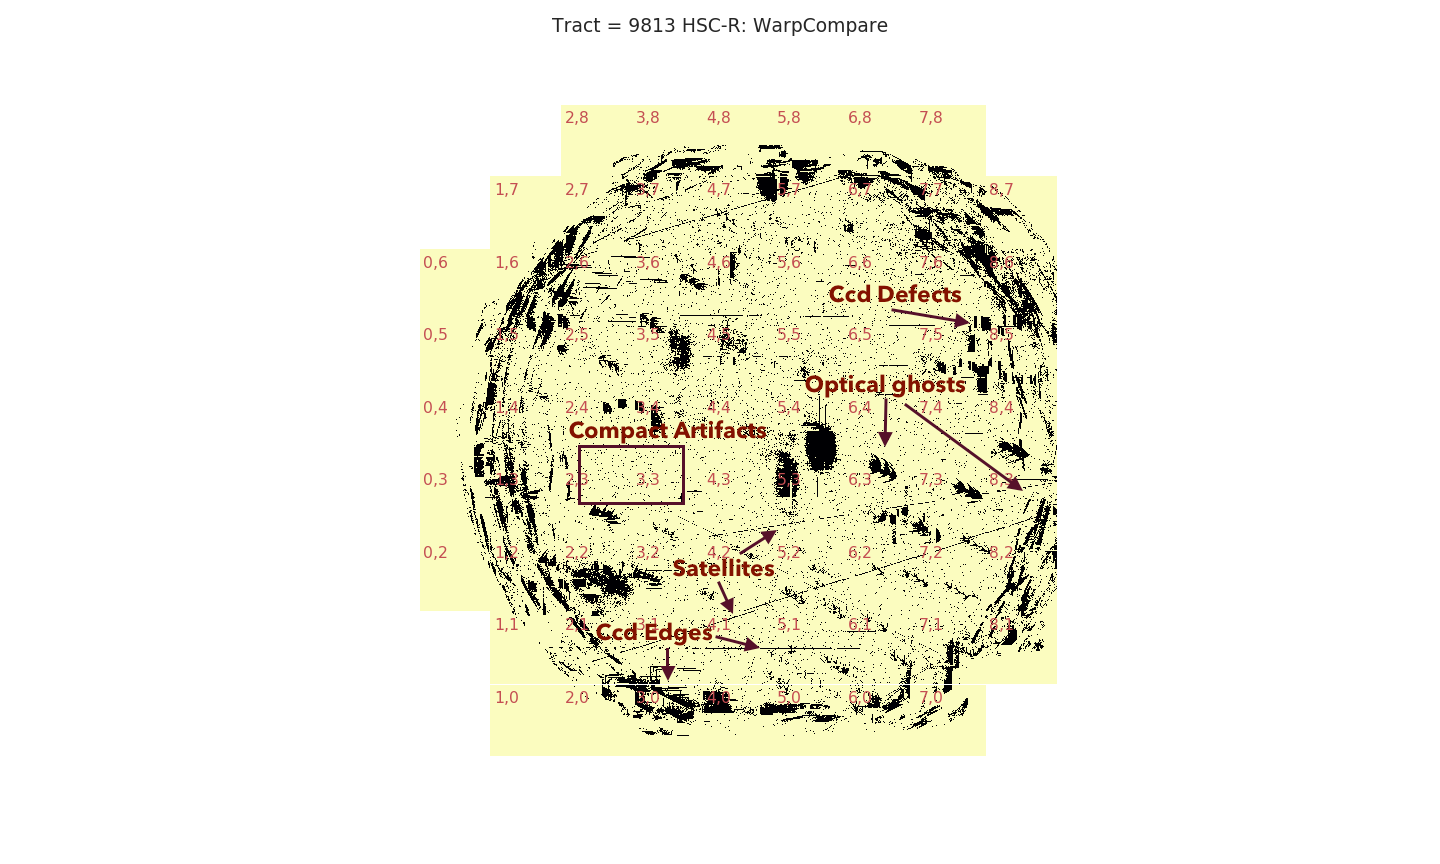
\includegraphics[clip,trim={.25\wd0} {.05\wd0} {.25\wd0} 0, width=0.30\textwidth]{figures/mask_DM-13637_9813HSC-R.png}
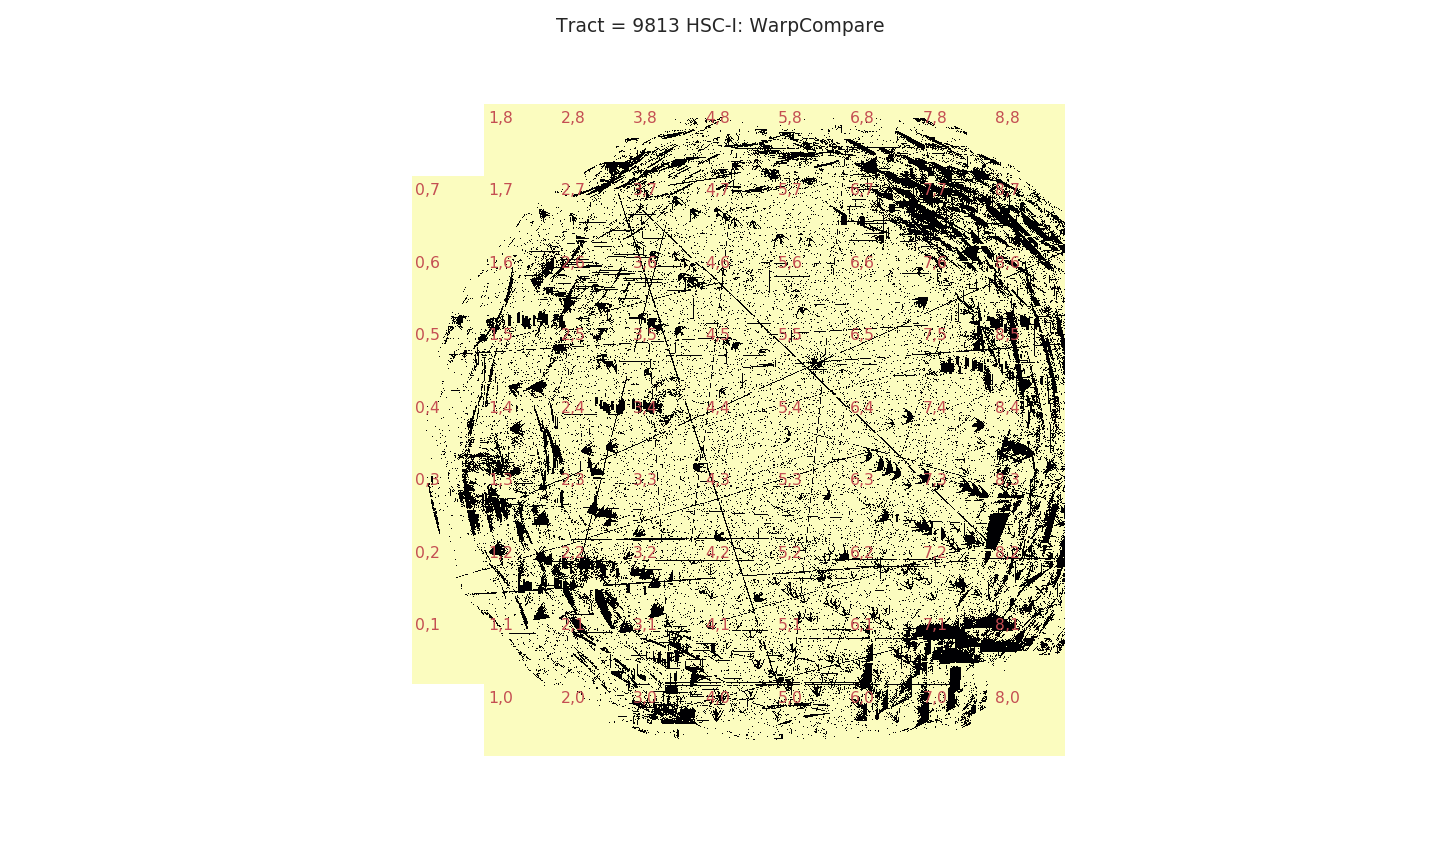
\includegraphics[clip,trim={.25\wd0} {.05\wd0} {.25\wd0} 0, width=0.30\textwidth]{figures/mask_DM-13637_9813HSC-I.png}
\\
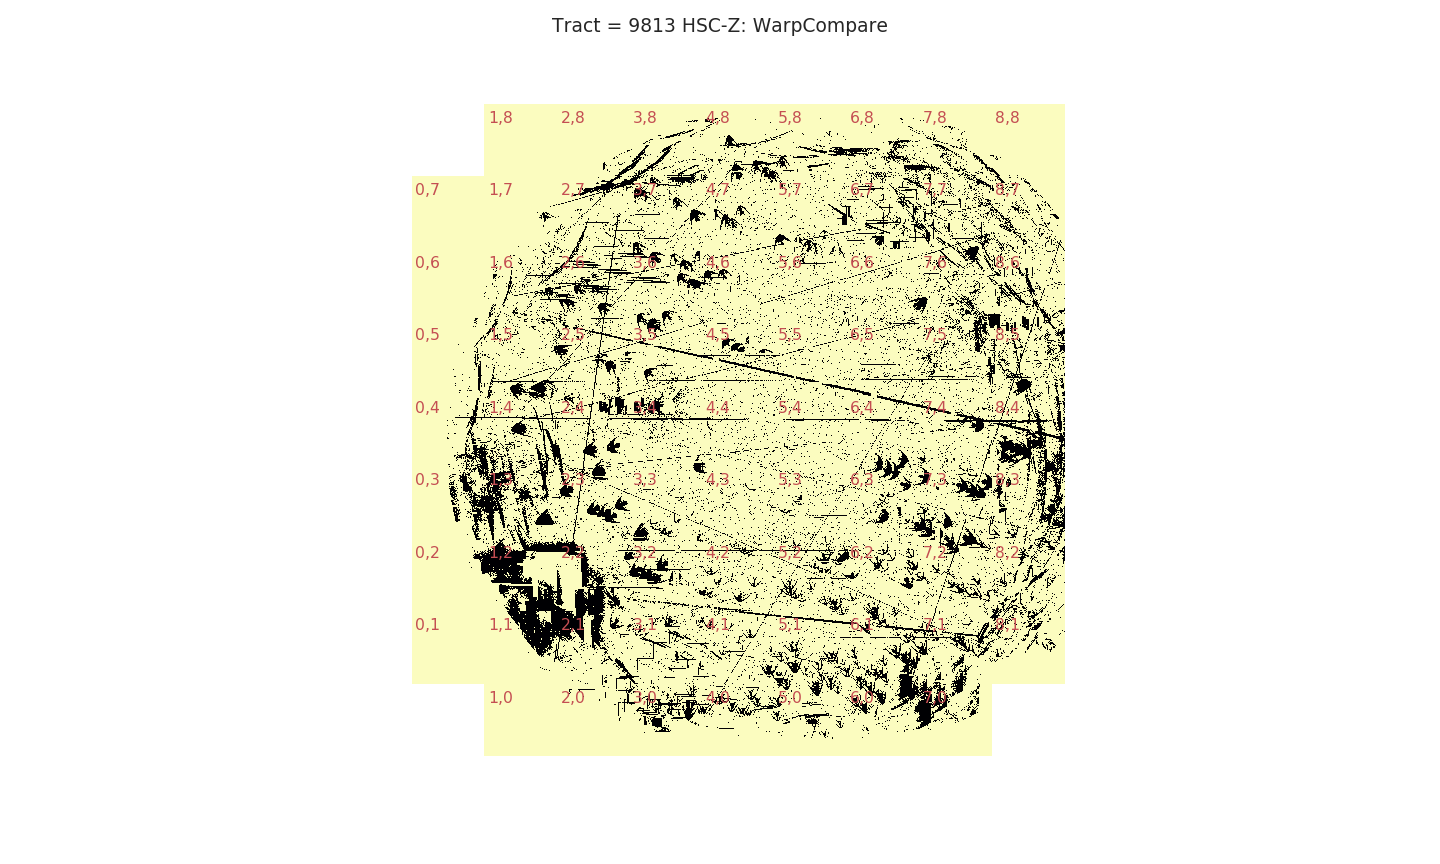
\includegraphics[clip,trim={.25\wd0} {.1\wd0} {.25\wd0} 0, width=0.48\textwidth]{figures/mask_DM-13637_9813HSC-Z.png}
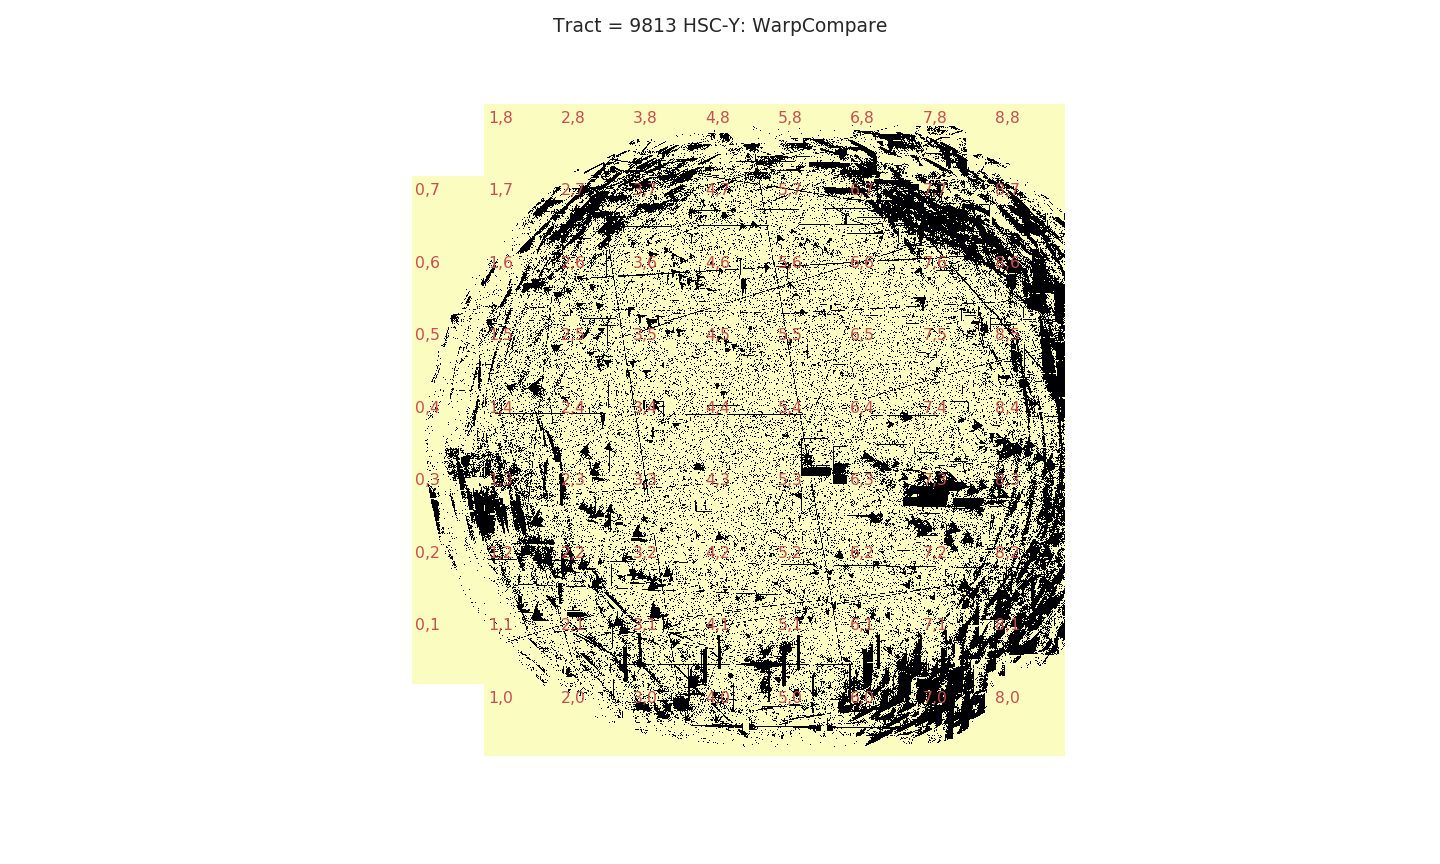
\includegraphics[clip,trim={.25\wd0} {.1\wd0} {.25\wd0} 0, width=0.48\textwidth]{figures/mask_DM-13637_9813HSC-Y.png}
\endgroup
\par\end{centering}
\caption{\label{fig:9813Maps} Masked pixels in tract 9813 for rerun \texttt{w\_2018\_18},  are shown in black. The red numbers label the upper lefthand corner of each patch within the tract. In patch 1,2 and 2,2 of HSC-Z (bottom left) there is a region where nothing is clipped because the pointings were dithered on scales smaller than those of the artifacts which overlapped from epoch to epoch.  Visible in these masks are satellite trails, optical ghosts, compact artifacts (e.g. asteroids, cosmic rays), and chip defects.}
\end{figure}

\section{Future Improvements}

\subsection{Background Matching}
\label{sec:background_matching}

The S18A  HSC data release included a new sky subtraction method designed to prevent the over-subtraction of the background around bright galaxies.
This background adjustment adds minor offsets in backgrounds from visit to visit, and these offsets degrade the quality of the warped image differencing during artifact rejection.
This effects \emph{in all existing artifact rejection algorithms in the stack}.
Background offsets in images being differenced increase false positives.

\begin{figure}
\begin{centering}
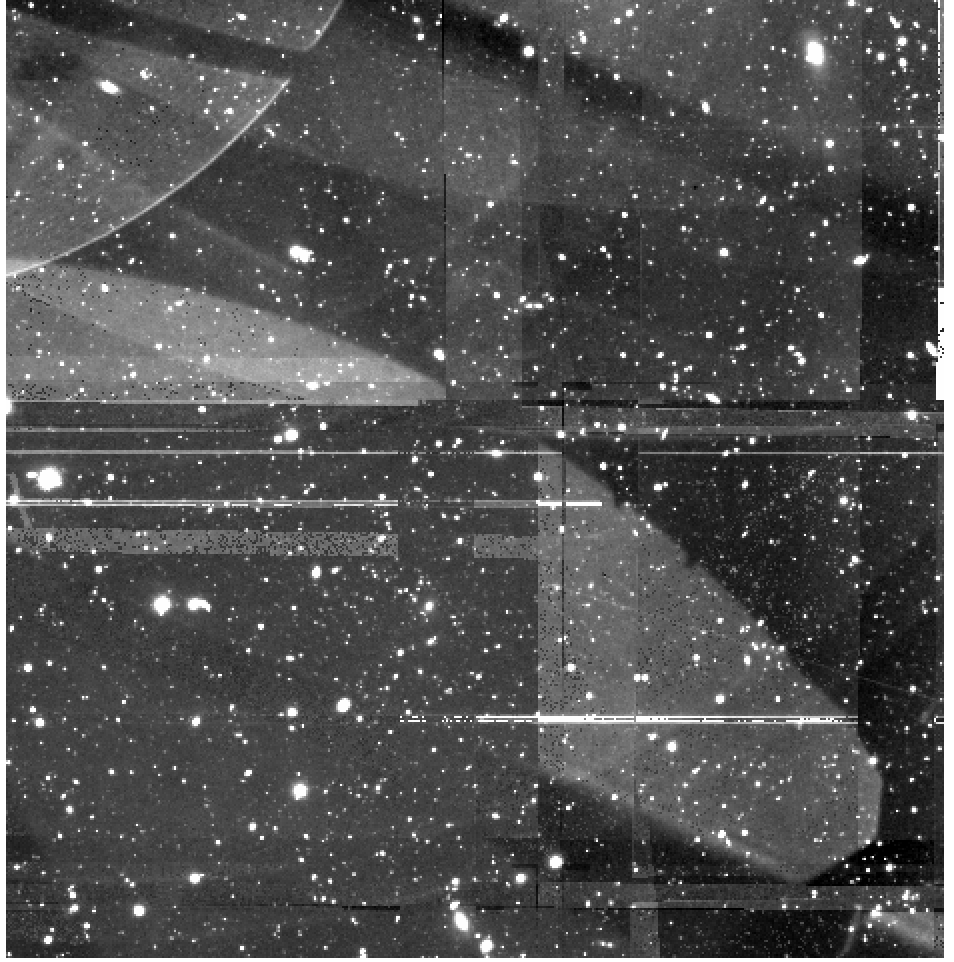
\includegraphics[width=0.3\textwidth]{figures/templateWBackgrounds.png}
\par\end{centering}
\caption{\label{fig:backgroundOffsets}  A sigma-clipped coadd for a problematic patch in the WIDE survey.  Background offsets caused by bright ghosts and the SkyCorrection algorithm interfere with the artifact rejection's differencing procedure which assumes backgrounds have been subtracted. Background matching will be necessary to mitigate the temporal background offsets.}
\end{figure}

\texttt{CompareWarpAssembleCoadd}  assumes that the backgrounds have been either subtracted or matched, and that they do not have large regions with offsets.
 Currently, \texttt{CompareWarpAssembleCoadd}  will handle regions with large background offsets in one of two ways.
 First, if the offsets are so ubiquitous that they appear in the template (as in the example shown in figure \ref{fig:backgroundOffsets}), then they cannot be clipped.
 If only a small fraction of visits are outliers  (and, significantly, at least 5$\sigma$ away from the static sky model), then they will be clipped.
 However, clipping large swaths of a patch is not ideal; a significant percentage of sources will have a PSF that is inexactly described by the coaddPSF.

The future planned implementation of background matching will significantly improve the fidelity of artifact candidate detection.

\section{Discussion}

In summary, while the \texttt{CompareWarp} algorithm has room for improvement, it performs better than \texttt{SafeClip} in terms of both false positives and false negatives.
This means there is no accuracy trade-off in using it as the artifact rejection algorithm.
\texttt{CompareWarp} can be used for all flavors of coadds
The only trade-off is the extra CPU time needed to produce PSF-matched warps.
Therefore, we propose making it the default coaddition algorithm in the stack.

% Include all the relevant bib files.
% https://lsst-texmf.lsst.io/lsstdoc.html#bibliographies
\bibliography{local,lsst,lsst-dm,refs_ads,refs,books}

\end{document}
